\chapter{Matrix representation of a winding}
In this section it will be shown that the winding layouts can be represented by means of two matrices. The first matrix will contain information on the ingoing coil sides of the coils while the second matrix will be that of the outgoing coil sides. The matrices are referred to as $\mathbf{M_1}$ and $\mathbf{M_{2}}$ for the ingoing and outgoing coil sides respectively. Both matrices have $n$ columns and $m$ rows. In addition, the number of columns equals the number of stator slots and the rows are equal to the number of phases, thus $m=m$\footnote{It is typical in mathematics that the number of rows is represented by $m$. Equally the number of phases of an electrical machine is also represented by $m$. Furthermore, $m_{11}$ is a matrix element while $m$ is the number of phases.} and $n=Q_s$. The matrices can be expressed as
\begin{equation}
  \label{eqn:M_matrix}
  \mathbf{M}_k = \left[
  \begin{array}{cccc}
     m_{11} & m_{12} & \ldots & m_{1n}\\
     m_{21} & m_{22} & \ldots & m_{2n}\\
     \vdots & \vdots & \ddots & \vdots\\
     m_{m1} & m_{m2} & \ldots & m_{mn}\\
  \end{array} \right]
  \qquad \mbox{where} \qquad
  \begin{cases}
     k = 1,2\\
     m_{ij} \in \left\{-1,0,1\right\}\\
  \end{cases}
\end{equation}
and depends on the winding layout. In the rest of this section an algebraic method is derived to determine the matrix elements. The variables $n_1$ and $n_2$ are integers and will be used as loop variables later on in this chapter where the algorithm flowchart is explained. The subscripts $1$ and $2$ refer to the outer and inner loop respectively. 

\section{Slot vector}
For assigning the $Q_s$ slots to phase belts, the peripheral slot angle $\alpha$ needs to be defined in terms of the slot pitch $\tau_s$. If the slots have a regular distribution the angle between any two adjacent slots equals $\tau_s$. In the case of irregular distributed slots the average slot pitch will equal $\tau_s$. A regular and irregular distribution are shown in Fig.~\ref{fig:f_slotstar}. A vector is assigned to the centre of each stator slot. The exponential representation\footnote{Also known as Euler's formula, \cite{REF-01047}.} of a vector is used, i.e.
\begin{equation} 
  e^{\i\nu \alpha}=\cos(\nu \alpha)+\i\sin(\nu \alpha)
\end{equation}
The variables $\nu$ and $\alpha$ are the harmonic order and slot peripheral angle respectively. All the vectors as shown in Fig.~\ref{fig:f_slotstar} are represented as a column matrix $\mathbf{v}_{\nu}$. The number of rows is equal to the number of slots, i.e.
\begin{equation}
  \label{eqn:slot_vector}
  \mathbf{v}_{\nu}=\left[
                         e^{\i\nu\alpha_1} 
                         \: 
                         e^{\i\nu\alpha_{n_2}} 
                         \:
                         \ldots 
                         \: e^{\i\nu\alpha_{Q_s}}
                    \right]^{T}
   \qquad 1 \leq n_2 \leq Q_s                 
\end{equation}
where
\begin{equation}
  \label{eqn:slot_alpha}
  \alpha_{n_2} = \left\{ \begin{array}{lll}
    \tau_s\left(n_2-1\right) && n_2 \;\text{odd}\\
    \alpha_{n_2-1}+x\tau_s & 0<x<2 & n_2\;\text{even}
  \end{array} \right.
  \quad
  1 \leq n_2 \leq Q_s
\end{equation}
where the $\alpha$ accounts for both regular and irregular distributed stator slots. Setting $\nu=p$ means that the electrical slot angles\footnote{The electrical and mechanical slot have the following relationship: $\theta_e=p \theta_m$} for the working harmonic are obtained. 
\begin{figure}
  \centering
  \fontsize{8}{0}\selectfont
  \subfloat[Regular distribution $x=1$\label{fig:slotstara}]{
  \begin{psfrags}%
\psfragscanon

% text strings:
\psfrag{t01}{1}
\psfrag{t02}{$Q_s$}
\psfrag{t03}{$2\tau_s$}
\psfrag{t04}{$x\tau_s$}

% Figure:
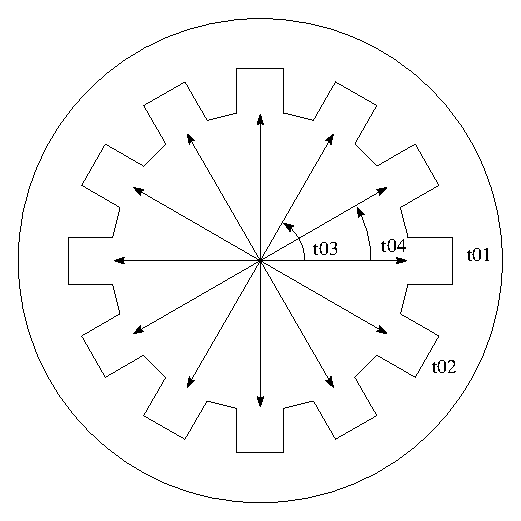
\includegraphics[height=6.5cm]{figs/f_slotstara.eps}
\end{psfrags}%
}
  \hfill
  \subfloat[Irregular distribution $0<x<2$\label{fig:slotstarb}]{
  \begin{psfrags}%
\psfragscanon

% text strings:
\psfrag{t01}{1}
\psfrag{t02}{$Q_s$}
\psfrag{t03}{$2\tau_s$}
\psfrag{t04}{$x\tau_s$}

% Figure:
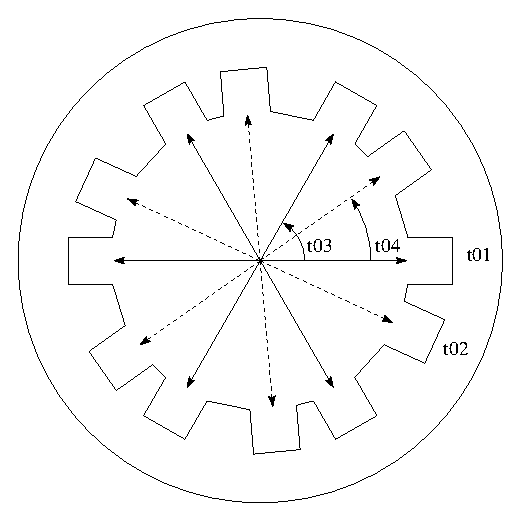
\includegraphics[height=6.5cm]{figs/f_slotstarb.eps}
\end{psfrags}%
}
  \caption{Star of slots}
  \label{fig:f_slotstar}
\end{figure}

\subsection{Phase belt constraint}
The phase belt constraint is used to determine the matrix elements $m_{ij}$ in \eqref{eqn:M_matrix}. From the slot angle $\alpha$ in \eqref{eqn:slot_vector} the corresponding electrical angle $\theta_e$ is obtained. A stator slot is assigned to the phase belt if the following constraint is true:
\begin{equation}  
 \label{eqn:phase_belt_constraint}
  \theta_1 \leq \theta_e  < \theta_2
  \quad
  \begin{cases}
    \left.
      \begin{array}{l}
        \theta_1 = \frac{2\pi}{2m}\left(n_1-1\right) \\
        \theta_2 = \frac{2\pi}{2m}n_1 \\
        1 \leq n_1 \leq N_p \\      
      \end{array}
    \right\} 
    \quad \mbox{phase belt boundaries} \\
    \left.
      \begin{array}{l}
        \theta_e = p\alpha_{n_2} \\
        1 \leq n_2 \leq Q_s \\      
      \end{array}    \right\} 
    \quad \mbox{electrical slot angle} \\
  \end{cases}
\end{equation} 
The phase belt constraint as given in \eqref{eqn:phase_belt_constraint} is characterised by the phase belt boundaries and the electrical slot angle, which are summerised as follows:
\begin{description}
  \item[Phase belt boundaries:] The total number of phase belts around the air gap~%
  periphery is given by \eqref{eqn:Np}. Each of the phase belts is bounded the by~%
  the angles $\theta_1$ and $\theta_2$.
  \item[Electrical slot angle:] The electrical slot angle is obtained by multiplying~%
  the peripheral slot angle in \eqref{eqn:slot_alpha} by the pole pair number. If~%
  the electrical angle for a given slot lies within the phase belt boundaries, it~%
  belongs to that phase belt.   
\end{description}
In order to assign the slot to a phase, it is necessary to know to which phase a given phase belt belongs. The phase can be determined in terms of the given phase belt number $n_1$ and the number of phases, i.e.
\begin{equation}
  \label{eqn:phase_belt_number}
  k = \mbox{mod}(n_1,2m)
  \quad
  \begin{cases}
    1 \leq n_1 \leq \ N_p \\
    2m \ \mbox{if} \ \mbox{mod}(n_1,2m)=0 \\
  \end{cases}
  \quad
  1\leq k \leq 2m
\end{equation}  
The value of $k$ as calculated in \eqref{eqn:phase_belt_number} corresponds to the phase belt number. Therefore, if the number of a given phase belt is known, the corresponding phase and its sign are calculated as follows:
\begin{equation}
  \label{eqn:phase_belt_number_2}
  \begin{aligned}
  \mbox{phase}&= 
    \left\{
    \begin{array}{ll}
      k   & k \leq m\\
      k-m & k > m
    \end{array}
    \right.
    \\
  \mbox{sign}&=(-1)^{(k-1)} 
  \end{aligned}
\end{equation}  
If $m=3$ and $p=1$ the number of phase belts equals 6. Applying \eqref{eqn:phase_belt_number} and \eqref{eqn:phase_belt_number_2} will result in the phase belt sequence as given in \eqref{eqn:phasebelt_sequence}. 

\subsection{Algorithm flowchart}
The explanation of the algorithm is accompanied by the flowchart in Fig.~\ref{fig:flowchart} and greatly simplifies the understanding. For convenience the relevant equations or tables are included which makes it easier to follow the description. The algorithm only applies to symmetrical windings and the three major parts are summerised as follows:
\begin{description}
\item[Outer loop:] The outer loop of the flowchart is used for the total number of phase belts as given in \eqref{eqn:Np}. The loop index $n_1$ (in the range $1\leq n_1 \leq N_p$) is used to calculate the given phase belt boundaries $\theta_1$ and $\theta_2$ as given in \eqref{eqn:phase_belt_constraint}. Since the $2m$ phase belts repeat themselves along the air gap periphery, the actual phase belt number $k$ in the phase belt sequence can be determined from $n_1$ as given in \eqref{eqn:phase_belt_number} and \eqref{eqn:phase_belt_number_2}.
\item[Inner loop:] The inner loop has $n_2$ as index and is used to calculate the electrical angle for a given slot. If a slot is already assigned to a phase belt, the winding matrix will have an entry in the set $\{-1,1\}$. In this case the loop is skipped. Another case where the loop is skipped is that of single layer fractional slot windings with a coil pitch greater than one (non-overlapping). In such a case only the odd numbered slots are assigned, i.e.
\begin{equation}\label{eqn:modn20}
  \mbox{skip loop if} \; \mbox{mod}(n_2,2) = 0 
  \quad 
  \forall
  \quad
  \begin{cases}
    n_l = 1    \\
    q_d > 1    \\
    y_d > 1
  \end{cases}
\end{equation} 
\item[Phase belt constraint:] This is the key step to allocate a stator slot. If the electrical angle lies within the phase belt boundaries, it belongs to the given phase belt. The row and column number for the ingoing matrix $\mathbf{M_1}$ are determined from the inner loop index $n_2$ and the given phase belt number. The row number for $\mathbf{M_2}$ is the same as for $\mathbf{M_1}$ and the column number is obtained from the coil pitch $y_d$.
\end{description}
The assignment of the stator slots as offered in this dissertation is unique and not presented in this way by any of the references consulted. 
\begin{figure}
  \centering
  \fontsize{9}{10}\selectfont
  \begin{psfrags}%
\psfragscanon

% text strings:
\psfrag{t01}[bc]{$n_1 = 1,N_p$}
\psfrag{t02}[bc]{$\theta_1, \; \theta_2$}
\psfrag{t04}[bc]{$k=f(n_1,m)$}
\psfrag{t05}[bc]{$n_2 = 1,Q_s$}
\psfrag{t07}[bc]{$\theta_1 \leq \theta_e < \theta_2$}
\psfrag{t08}[bc]{$i=f(k)$ and $h=-1^{(k-1)}$}
\psfrag{t09}[bc]{$\mathbf{M}_{1,ij}=h \quad j=n_2$}
\psfrag{t10}[bc]{$\mathbf{M}_{2,ij}=-h \quad j=f(n_2,y_d)$}
\psfrag{t11}[bc]{$n_2=Q_s$?}
\psfrag{t12}[bc]{$n_1=N_p$?}
\psfrag{t14}[bc]{Start}
\psfrag{t15}[bc]{$\mathbf{M}_{ij} \in \left\{-1,1\right\}$}

\psfrag{t16}[bc]{$\mbox{mod}(n_2,2)=0$}
\psfrag{t161}[bc]{\eqref{eqn:modn20}}
\psfrag{t18}[br]{Slots}
\psfrag{t19}[br]{Phase belts}

\psfrag{t20}[bc]{$\theta_e = f(\tau_s)$}
\psfrag{t21}[bl]{\eqref{eqn:phase_belt_number}}

\psfrag{t23}[bl]{\eqref{eqn:Np}}

\psfrag{t13}[bc]{End}
\psfrag{t29}[br]{Section \ref{sec:m_assignment}}
\psfrag{t30}[bl]{\eqref{eqn:phase_belt_constraint}}
\psfrag{t32}[bl]{\eqref{eqn:matrix_element}}
\psfrag{t33}[bc]{y}
\psfrag{t34}[bc]{n}

% Figure:
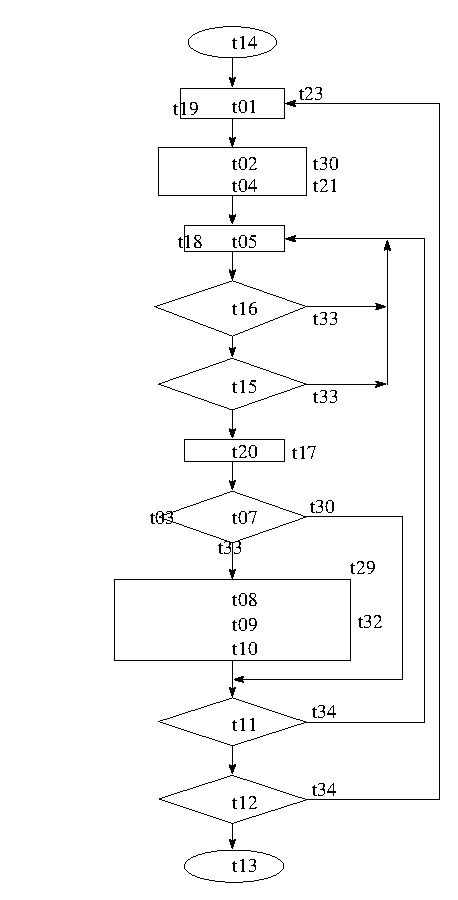
\includegraphics[width=0.55\textwidth]{figs/f_flowchart.eps}
\end{psfrags}%
  \caption{Flowchart to allocate the stator slots}
  \label{fig:flowchart}
\end{figure}

\subsection{Matrix element assignment}\label{sec:m_assignment}
Once the phase belt constraint is fulfilled, the slot is allocated and the next step is to assign one of the values in the set given in \eqref{eqn:M_matrix}. Actually only the sign needs to be determined. Since the phase belt sequence is alternating, the sign can be obtained from the phase belt itself. Following the flowchart through to the point where the test is performed, it is noticed that the matrix column number for $\mathbf{M}_1$ is given by the loop index variable $n_2$. The entry has the value  $(-1)^{(k-1)}$, where $k$ is given in \eqref{eqn:phase_belt_number}. The determination of the row, column and matrix element are summerised as follows\footnote{The method was only tested for $m=3,5,7,\ldots$}: 
\begin{equation}
  \label{eqn:matrix_element}
  \begin{aligned}
  i &= 
  \left\{ 
    \begin{array}{ll}
      k   & k \leq m\\
      k-m & k > m
    \end{array}
    \qquad 
  \right\}
  \mbox{row number}
  \\
  h &= (-1)^{(k-1)} 
  \quad 
  \mbox{matrix element sign} 
  \\
  j &= 
  \left\{ 
    \begin{array}{ll}
      n_2+y_d   & n_2+y_d \leq Q_s \\
      \mbox{mod}\bigl((n_2+y_d),Q_s\bigr) & n_2+y_d > Q_s
    \end{array} 
    \quad
  \right\}
  \mbox{column number}
  \end{aligned}
\end{equation}

\section{Properties of the winding matrix}
Presenting the winding in matrix form is very compact and has advantages in machine analysis. The matrix contains all the information of the winding arrangement in the stator slots. This allows the construction of the voltage phasor which is necessary to calculate the winding factor. In addition, the slot mmf can be obtained from the column data. The properties of the matrix are summerised as follows:
\begin{itemize}
  \item if the winding is symmetrical, the number of assigned elements in all~%
  the rows are equal;
  \item the number of columns is equal to the number of stator slots;
  \item the number of rows is equal to the number of phases;
  \item for a single layer winding there is only one nonzero element in a column;
  \item a double layer winding has two nonzero elements in a row; and
  \item the matrix is valid for both a fixed and variable slot pitch.
\end{itemize}
In the rest of this section the winding matrix is used to calculate the winding factor and the slot mmf.

\subsection{Winding factor}
With $\mathbf{M}_1$ and $\mathbf{M}_2$ assigned, the winding factor for any harmonic can be calculated as the product between the matrices and the slot vector as given in \eqref{eqn:slot_vector}. This means that a row of the winding matrix is multiplied by the slot vector column matrix. The matrix product means that all the vectors belonging to the same phase are added and for the case $\nu=p$ equals\footnote{$j$ as imaginary number and $j$ as column number can be confusing.}
\begin{equation}
  \label{eqn:m1_m2_exp}
  c_{i1}e^{\i p\alpha_1}+c_{i2}e^{\i p\alpha_2}+\ldots+
  c_{iQ_s}e^{\i p \alpha_{Q_s}} = \sum_{j=1}^{Q_s}c_{ij}e^{\i p\alpha_k}
  \quad \mbox{where} \quad
  c_{ij} = m_{1,ij}+m_{2,ij}
\end{equation}
If the slot vector does not belong to the current phase, the coefficient
\begin{equation} 
  \left(m_{1,ij}+m_{2,ij}\right)
\end{equation} 
is zero. Furthermore, the product should be normalised. Since the total number of vectors is related to the coils per phase it should be multiplied by $\left(2\frac{Q_c}{m}\right)^{-1}$, i.e.
\begin{equation}
  \label{eqn:winding_factor}
  \xi_{\nu} = \frac{m}{2Q_c}
  \Bigl[
    \mathbf{M}_1\mathbf{v_{\nu}}+\mathbf{M}_2\mathbf{v_{\nu}}
  \Bigr], 
  \quad \in \mathbb{C}
\end{equation}
The result \eqref{eqn:winding_factor} present the winding factor as a complex number and the absolute value is to be used as a reduction factor for the sinusoidally induced voltage in \eqref{eqn:ui}. Writing $\xi_{\nu}$ as
\begin{equation}
  \xi_{\nu} = a_{\nu}+\i b_{\nu}
\end{equation}
the phase angle is calculated as 
\begin{equation}
  \theta_{\nu} = \arctan\left(\frac{b_{\nu}}{a_{\nu}}\right)
\end{equation}
The phase angle (in electrical radians) gives information on the position of the winding axes\footnote{The winding axes in the present dissertation refer to the current anti-node axis and the magnetic axis.} relative to the first slot. The two winding axes associated with each phase are called (a) the current sheet anti-node axis; and (b) the magnetic axis of the winding. A positive phase angle means that both winding axes have moved clockwise with respect to the first slot. The winding axes are a very import quantities in machine design. When the machine is supplied with a source, a rotating magnetic flux wave is generated. This reacts with the flux generated by the flux of the permanent magnets on the rotor. In order to control the resultant flux, it is necessary to know the exact position of the winding axes.  
\index{current sheet anti-node axis}
\index{magnetic axis}

\begin{equation}\label{eqn:dft}
  X(k) = \sum_{j=1}^N \; x(j) \; e^{-(j-1)(k-1)\theta i}
  \qquad
  \xi(\nu) = \sum_{k=1}^{Q_s}c_{ik}e^{jp\alpha_k}
\end{equation}

\subsection{Current sheet anti-node axis}\label{subsec:current_sheet}
Equation \eqref{eqn:F_theta_t_1} describes the space fundamental component of the mmf produced by the current in phase 1. It can be seen as the mmf wave produced by a finely divided sinusoidally distributed current sheet placed on the inner periphery of the stator. The position of the anti-node with maximum deviation is given by $\theta_{an}$. The relative position of $\theta_{an}$ with respect to the first slot is given by
\begin{equation}
  \label{eqn:theta_an}
  \theta_{an_{\nu}} = -
  \frac{\theta_{\nu}}{p}
\end{equation} 

\subsection{Magnetic axis}\label{subsec:magnetic_axis}
The axis along which the flux is directed when current is flowing in the coil, is defined as the magnetic axis. This is the same position where the current sheet has a node. The relative position of the magnetic axis $\theta_m$ with respect to the first slot is given by
\begin{equation}
  \label{eqn:theta_m}
  \theta_{m_{\nu}} = -
  \frac{\left(\theta_{\nu}+\frac{\pi}{2}\right)}{p}
\end{equation} 
The winding magnetic axis lags the current sheet anti-node axis by $\frac{\pi}{2}$
radians.

\subsection{Slot mmf}\label{subsec:slot_mmf}
The amp\`ere-turns in each slot can be obtained from the matrix winding columns. Both the matrices $\mathbf{M_1}$ and $\mathbf{M_2}$ contain the coil side information for the ingoing and outgoing coil sides respectively. The total amp\`ere-turns of a coil side is the product of its value in the winding matrix with the number of coil turns $N_t$. The direction of the current is given by the sign of the element. Therefore to get the total amp\`ere-turns in the slot, the amp\`ere-turns of the coil sides must be added. For a three-phase winding the slot mmf $F_{slot}$ of the $k^{th}$ slot is calculated as  
\begin{equation}
  \label{eqn:slot_mmf}
  \begin{aligned}
  F_{slot,k} &= N_t i_1(m_{1,1k}+m_{2,1k})+
                N_t i_2(m_{1,2k}+m_{2,2k})+
                N_t i_3(m_{1,3k}+m_{2,3k}) \\
             &= N_t\sum_{n=1}^{3}i_n \left(m_{1,nk}+m_{2,nk}\right) 
  \end{aligned}
\end{equation}

\section{Examples}
The derived theory presented in this chapter is now illustrated by means of examples. The examples are summerised as follows:
\begin{description}
  \item[Winding factor tables:] The winding factors for different slot and pole pair combinations are calculated for single and double layer non-overlapping windings. The results presented are used to derive an expression to find the feasible range for the number of pole pairs, given the number of stator slots. 
  \item[Slot mmf and current sheet:] The prototype stator with 30 slots is used as an example. By choosing different pole pair numbers, it is shown how to obtain both a single and double layer winding. In each case a non-overlapping and overlapping winding are explained.
\end{description}
  
\subsection{Winding factor table}\label{subsec:wind_fac_table}
The results are given in Tab.~\ref{tab:xi_single} Tab.~\ref{tab:xi_double} for single and double layer non-overlapping windings respectively. Only those slot and pole combinations for which the winding factor is greater than or equal to $\frac{\sqrt{3}}{2}$ are given. Those combinations that do not fulfill the condition in \eqref{eqn:feasibility} are marked as not applicable. Presenting the winding factors in a table is helpful to identify the relationship between the number of stator slots and the number of poles which results in the best combinations. Only the winding factors for the working harmonic are presented. 

The winding factors for single windings are calculated for pole pairs in the range from 4 to 28, whereas the number of stator slots range from 12 to 84. Although the focus in the present dissertation is on single layer non-overlapping windings, the winding factors for double layer windings are given as well. The winding factors are calculated for pole pairs in the range from 4 to 16, whereas the number of stator slots ranges from 12 to 48.
\begin{table}[htbp]
  \caption{$\xi_p \times \num{e-3}$ for single layer non-overlapping windings}
  \label{tab:xi_single}
  \centering
   \begin{tabular}
  	{|l||c|c|c|c|c|c|c|c|c|c|c|c|c|}\cline{2-14}
  	\multicolumn{1}{c}{}& \multicolumn{13}{|c|}{$Q_s$}
  	\\\hline
  	$p$&12 &18 &24 &30 &36 &42 &48 &54 &60 &66 &72 &78 &84  \\\hline
  	4  &866&   &   &   &   &   &   &   &   &   &   &   &    \\
  	5  &966&   &   &   &   &   &   &   &   &   &   &   &    \\
  	6  &na &866&   &   &   &   &   &   &   &   &   &   &    \\
  	7  &966&902&   &   &   &   &   &   &   &   &   &   &    \\
  	8  &866&945&866&   &   &   &   &   &   &   &   &   &    \\
  	9  &   &na &na &   &   &   &   &   &   &   &   &   &    \\
  	10 &   &945&966&866&   &   &   &   &   &   &   &   &    \\
  	11 &   &902&958&874&   &   &   &   &   &   &   &   &    \\
  	12 &   &866&na &na &866&   &   &   &   &   &   &   &    \\
  	13 &   &   &958&940&870&   &   &   &   &   &   &   &    \\
  	14 &   &   &966&950&na &866&   &   &   &   &   &   &    \\
  	15 &   &   &na &na &966&na &   &   &   &   &   &   &    \\
  	16 &   &   &866&950&na &na &866&   &   &   &   &   &    \\
  	17 &   &   &   &940&956&na &859&   &   &   &   &   &    \\
  	18 &   &   &   &na &na &na &na &866&   &   &   &   &    \\
  	19 &   &   &   &866&956&na &907&na &   &   &   &   &    \\
  	20 &   &   &   &866&na &na &966&na &866&   &   &   &    \\
  	21 &   &   &   &   &966&na &na &na &na &   &   &   &    \\
  	22 &   &   &   &   &na &na &958&na &954&866&   &   &    \\
  	23 &   &   &   &   &870&na &956&na &893&na &   &   &    \\
  	24 &   &   &   &   &866&na &na &na &na &na &866&   &    \\
  	25 &   &   &   &   &   &na &956&na &966&na &848&   &    \\
  	26 &   &   &   &   &   &na &958&na &na &na &870&866&    \\  
  	27 &   &   &   &   &   &na &na &na &na &na &na &na &    \\  
  	28 &   &   &   &   &   &866&966&na &na &na &na &na &866 \\\hline  	  
  \end{tabular}
\end{table}
 
\begin{table}[htbp]
  \caption{$\xi_p \times \num{e-3}$ for double layer non-overlapping windings }
  \label{tab:xi_double}
  \centering
  \begin{tabular}
  	{|l||c|c|c|c|c|c|c|c|c|c|c|c|c|}\cline{2-14}
  	\multicolumn{1}{c}{}& \multicolumn{13}{|c|}{$Q_s$}
  	\\\hline
  	$p$&12 &15 &18 &21 &24 &27 &30 &33 &36 &39 &42 &45 &48  \\\hline
  	4  &866&   &   &   &   &   &   &   &   &   &   &   &    \\
  	5  &930&866&   &   &   &   &   &   &   &   &   &   &    \\
  	6  &na &na &866&   &   &   &   &   &   &   &   &   &    \\
  	7  &930&950&900&866&   &   &   &   &   &   &   &   &    \\
  	8  &866&950&950&890&866&   &   &   &   &   &   &   &    \\
  	9  &   &na &na &na &na &866&   &   &   &   &   &   &    \\
  	10 &   &866&950&950&930&880&866&   &   &   &   &   &    \\
  	11 &   &   &900&950&950&920&870&866&   &   &   &   &    \\
  	12 &   &   &866&na &na &950&na &na &866&   &   &   &    \\
  	13 &   &   &   &890&950&950&940&900&870&866&   &   &    \\
  	14 &   &   &   &866&930&950&950&930&900&860&866&   &    \\
  	15 &   &   &   &   &na &950&na &na &930&na &na &866&    \\
  	16 &   &   &   &   &866&920&950&950&950&920&890&860&866 \\\hline  	  
  	\end{tabular}
\end{table}

From the results in Tab.~\ref{tab:xi_single} and Tab.~\ref{tab:xi_double} the number of slots per pole and phase which results in a winding with suitable winding factors is given by
\begin{equation}
  \frac{1}{4} \leq q \leq \frac{1}{2}
\end{equation}
The result is the same as presented by \cite{REF-00754} and \cite{REF-00756}. Using this result, the range of pole pairs for a given number of slots can be expressed as follows:
\begin{equation}
  \frac{Q_s}{m} \leq p \leq \frac{2Q_s}{m}
  \quad
  \left\{
  \begin{array}{ll}
  Q_s \in \left\{6,12,18,\ldots\right\} & \mbox{single layer}\\
  \:  & \: \\
  Q_s \in \left\{3,6,9,\ldots\right\} & \mbox{double layer}\\
  \end{array}
  \right.
\end{equation} 

\subsection{Slot mmf and current sheet}
This section entails examples of overlapping and non-overlapping windings with 30 stator slots. The classification parameters $q$, $q_c$ and $y_d$ (as given in Tab.~\ref{tab:Example_table}) are used to classify the windings according to the scheme in Fig.~\ref{fig:classification}. Additionally, for the selected number of pole pairs the winding factor, slot mmf and current sheet are calculated. It is important to mention that the choice of the position of the reference slot will determine the rotation direction of the resulting rotating field. It is desirable to have a field rotating in a counter-clockwise direction, since this is the positive direction in a polar coordinate system. To achieve this, the stator is rolled flat with the top part of the slots facing upwards. 
\begin{table}[htbp]
  \caption{Different pole pair combinations with $Q_s = 30$}
  \label{tab:Example_table}
  \centering  
   \begin{tabular}{ccccccccccccccccc}
    \toprule
  	$Q_s$ &$p$ &$Q_c$ &$n_l$& $y_p$ &$y_d$ &$q$ &$q_c$ & $Q_b$ & $t$ &
  	$\xi_p$ &$\xi_{5p}$ &$\xi_{7p}$ &Figure
  	\\
  	\midrule
  	30    &10  &15  &1   &$\frac{3}{2}$   &1   &$\frac{1}{2}$ &  $\frac{1}{4}$& 6 & 5 &
  	0.866   &0.866      &0.866      &%
  	\ref{fig:Main_non-overlapping_single}\subref{fig:f_Qs30_p10_1}
  	\\
  	30    &10  &30  &2    &$\frac{3}{2}$  &1   &$\frac{1}{2}$ &  $\frac{1}{2}$ & 3&10 &
  	0.866   &0.866      &0.866      &%
  	\ref{fig:Main_non-overlapping_double}\subref{fig:f_Qs30_p10_2}
  	\\    
  	30    &5   &15  &1    &3 &3  &1 &  $\frac{1}{2}$ & 6 & 5  &
  	1.0     &1.0        &1.0        &%
  	\ref{fig:Main_single_overlapping}\subref{fig:f_Qs30_5_1}
  	\\
  	30    &5   &30  &2    &3 &3  &1 &  1 & 6 & 5  &
  	1.0     &1.0        &1.0        &%
  	\ref{Main_double_overlapping}\subref{fig:f_Qs30_p5_2}   
  	\\
  	\bottomrule  	  
   \end{tabular}
\end{table} 

\subsubsection{Single layer non-overlapping}
Fig.~\ref{fig:Main_non-overlapping_single}\subref{fig:single_layer} shows an illustration of a single layer non-overlapping winding. There is only one coil side in each stator slot and the slot pitch could be either regular or irregular. An irregular slot pitch means that the coil pitch can be varied to improve the winding factor. Depending on the design criteria, it can also be used to improve the torque ripple. Since the outgoing coils are given by the coil pitch $y_d$, only every second slot needs to be assigned to a phase belt.  

The example chosen is that of the prototype machine with 30 slots and 10 pole pairs. 
From Tab.~\ref{tab:Example_table} the values for $q$ and $q_c$ are $\frac{1}{2}$ and $\frac{1}{4}$ respectively. The basic winding is determined using $q_c$ and has one  coil per phase distributed over 4 poles. In total the basic winding has 6 slots. The winding has a sub-harmonic with 5 pole pairs. Since it is a single layer winding the number of coils is half the number of stator slots. The coil pitch equals one and this is a fractional slot winding. For convenience only the basic winding matrix elements for $\mathbf{M_1}$ and $\mathbf{M_2}$ are given as
\begin{equation}
  \mathbf{M_{1,b}} = 
  \begin{pmatrix}
  1&0&0&0&0&0\\
  0&0&1&0&0&0\\
  0&0&0&0&1&0\\
  \end{pmatrix} \
  \mathbf{M_{2,b}} = 
  \begin{pmatrix}
  0&-1&0&0 &0&0 \\
  0&0 &0&-1&0&0 \\
  0&0 &0&0 &0&-1\\
  \end{pmatrix} 
\end{equation}
To obtain the complete winding matrix, the matrix of the basic winding is repeated five times. For the ingoing coil side matrix this means
\begin{equation}
  \mathbf{M_1} = 
  \begin{bmatrix}
  \mathbf{M_{1,b}}&\mathbf{M_{1,b}}&\mathbf{M_{1,b}}&
  \mathbf{M_{1,b}}&\mathbf{M_{1,b}}
  \end{bmatrix}  
\end{equation}
The winding matrix is used to obtain the slot mmf $F_{slot}$ from \eqref{eqn:slot_mmf} as shown in the lower part of~%
Fig.~\ref{fig:Main_non-overlapping_single}\subref{fig:f_Qs30_p10_1}. The dashed line in the mmf plot is the current sheet. In the top part of the figure the winding factors are shown as well. From the figure it is clear that the winding factors are periodic with the number of stator slots. In the example the peripheral slot angle was calculated setting $x=1$ in \eqref{eqn:slot_alpha}. Therefore, this is a regular distribution of the stator slots.
\begin{figure}[htbp]
  \centering
  \fontsize{6}{6}\selectfont
  \subfloat[Winding layout\label{fig:single_layer}]{
  \begin{psfrags}%
\psfragscanon

% text strings:
\psfrag{t01}{{\tiny Constant pitch, $2\tau_s$}}
\psfrag{t02}{{\tiny Variable slot pitch, $x \tau_s$}}
\psfrag{t03}{{\tiny Direction of coil assignment}}
\psfrag{t04}{{\tiny 1}}
\psfrag{t05}{{\tiny 2}}
\psfrag{t06}{{\tiny 3}}
\psfrag{t07}{{\tiny 4}}

% Figure:

\subfloat[Winding layout\label{fig:single_layer}]
  \hfill
  \subfloat[Slot mmf and winding factors\label{fig:f_Qs30_p10_1}]{
  % This file is generated by the MATLAB m-file laprint.m. It can be included
% into LaTeX documents using the packages graphicx, color and psfrag.
% It is accompanied by a postscript file. A sample LaTeX file is:
%    \documentclass{article}\usepackage{graphicx,color,psfrag}
%    \begin{document}% This file is generated by the MATLAB m-file laprint.m. It can be included
% into LaTeX documents using the packages graphicx, color and psfrag.
% It is accompanied by a postscript file. A sample LaTeX file is:
%    \documentclass{article}\usepackage{graphicx,color,psfrag}
%    \begin{document}% This file is generated by the MATLAB m-file laprint.m. It can be included
% into LaTeX documents using the packages graphicx, color and psfrag.
% It is accompanied by a postscript file. A sample LaTeX file is:
%    \documentclass{article}\usepackage{graphicx,color,psfrag}
%    \begin{document}\input{f_Qs_30_p_10_1}\end{document}
% See http://www.mathworks.de/matlabcentral/fileexchange/loadFile.do?objectId=4638
% for recent versions of laprint.m.
%
% created by:           LaPrint version 3.16 (13.9.2004)
% created on:           12-Nov-2008 21:44:16
% eps bounding box:     17.5 cm x 13.125 cm
% comment:              
%
\begin{psfrags}%
\psfragscanon%
%
% text strings:
\psfrag{s05}[b][b]{{\tiny $\xi_{10}$}}%
\psfrag{s06}[b][b]{{\tiny $\xi_{50}$}}%
\psfrag{s07}[b][b]{{\tiny $\xi_{70}$}}%
\psfrag{s08}[t][t]{{\tiny $\nu$}}%
\psfrag{s09}[b][b]{{\tiny $\xi_{\nu}$}}%
\psfrag{s10}[t][t]{{\tiny Slot number}}%
\psfrag{s11}[b][b]{{\tiny $F_{slot}/\SI{}{A}$}}%
%
% xticklabels:
\psfrag{x01}[t][t]{{\tiny 0}}%
\psfrag{x02}[t][t]{{\tiny 5}}%
\psfrag{x03}[t][t]{{\tiny 10}}%
\psfrag{x04}[t][t]{{\tiny 15}}%
\psfrag{x05}[t][t]{{\tiny 20}}%
\psfrag{x06}[t][t]{{\tiny 25}}%
\psfrag{x07}[t][t]{{\tiny 30}}%
\psfrag{x08}[t][t]{{\tiny 0}}%
\psfrag{x09}[t][t]{{\tiny 10}}%
\psfrag{x10}[t][t]{{\tiny 20}}%
\psfrag{x11}[t][t]{{\tiny 30}}%
\psfrag{x12}[t][t]{{\tiny 40}}%
\psfrag{x13}[t][t]{{\tiny 50}}%
\psfrag{x14}[t][t]{{\tiny 60}}%
\psfrag{x15}[t][t]{{\tiny 70}}%
\psfrag{x16}[t][t]{{\tiny 80}}%
\psfrag{x17}[t][t]{{\tiny 90}}%
%
% yticklabels:
\psfrag{v01}[r][r]{{\tiny -1}}%
\psfrag{v02}[r][r]{{\tiny -0.5}}%
\psfrag{v03}[r][r]{{\tiny 0}}%
\psfrag{v04}[r][r]{{\tiny 0.5}}%
\psfrag{v05}[r][r]{{\tiny 1}}%
\psfrag{v06}[r][r]{{\tiny 0}}%
\psfrag{v07}[r][r]{{\tiny 0.1}}%
\psfrag{v08}[r][r]{{\tiny 0.2}}%
\psfrag{v09}[r][r]{{\tiny 0.3}}%
\psfrag{v10}[r][r]{{\tiny 0.4}}%
\psfrag{v11}[r][r]{{\tiny 0.5}}%
\psfrag{v12}[r][r]{{\tiny 0.6}}%
\psfrag{v13}[r][r]{{\tiny 0.7}}%
\psfrag{v14}[r][r]{{\tiny 0.8}}%
\psfrag{v15}[r][r]{{\tiny 0.9}}%
\psfrag{v16}[r][r]{{\tiny 1}}%
\psfrag{v17}[r][r]{{\tiny 1.1}}%
%
% Figure:

\subfloat[Slot mmf and winding factors\label{fig:f_Qs30_p10_1}]{%
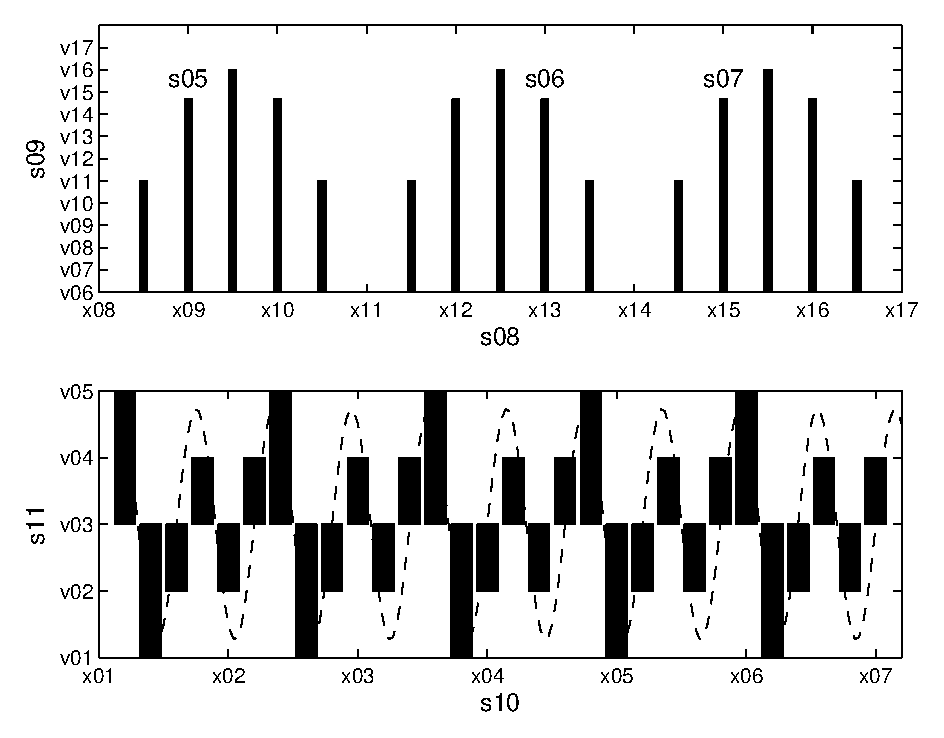
\includegraphics[width=0.9\textwidth]{figs/f_Qs_30_p_10_1.eps}}%
\end{psfrags}%
%
% End f_Qs_30_p_10_1.tex
\end{document}
% See http://www.mathworks.de/matlabcentral/fileexchange/loadFile.do?objectId=4638
% for recent versions of laprint.m.
%
% created by:           LaPrint version 3.16 (13.9.2004)
% created on:           12-Nov-2008 21:44:16
% eps bounding box:     17.5 cm x 13.125 cm
% comment:              
%
\begin{psfrags}%
\psfragscanon%
%
% text strings:
\psfrag{s05}[b][b]{{\tiny $\xi_{10}$}}%
\psfrag{s06}[b][b]{{\tiny $\xi_{50}$}}%
\psfrag{s07}[b][b]{{\tiny $\xi_{70}$}}%
\psfrag{s08}[t][t]{{\tiny $\nu$}}%
\psfrag{s09}[b][b]{{\tiny $\xi_{\nu}$}}%
\psfrag{s10}[t][t]{{\tiny Slot number}}%
\psfrag{s11}[b][b]{{\tiny $F_{slot}/\SI{}{A}$}}%
%
% xticklabels:
\psfrag{x01}[t][t]{{\tiny 0}}%
\psfrag{x02}[t][t]{{\tiny 5}}%
\psfrag{x03}[t][t]{{\tiny 10}}%
\psfrag{x04}[t][t]{{\tiny 15}}%
\psfrag{x05}[t][t]{{\tiny 20}}%
\psfrag{x06}[t][t]{{\tiny 25}}%
\psfrag{x07}[t][t]{{\tiny 30}}%
\psfrag{x08}[t][t]{{\tiny 0}}%
\psfrag{x09}[t][t]{{\tiny 10}}%
\psfrag{x10}[t][t]{{\tiny 20}}%
\psfrag{x11}[t][t]{{\tiny 30}}%
\psfrag{x12}[t][t]{{\tiny 40}}%
\psfrag{x13}[t][t]{{\tiny 50}}%
\psfrag{x14}[t][t]{{\tiny 60}}%
\psfrag{x15}[t][t]{{\tiny 70}}%
\psfrag{x16}[t][t]{{\tiny 80}}%
\psfrag{x17}[t][t]{{\tiny 90}}%
%
% yticklabels:
\psfrag{v01}[r][r]{{\tiny -1}}%
\psfrag{v02}[r][r]{{\tiny -0.5}}%
\psfrag{v03}[r][r]{{\tiny 0}}%
\psfrag{v04}[r][r]{{\tiny 0.5}}%
\psfrag{v05}[r][r]{{\tiny 1}}%
\psfrag{v06}[r][r]{{\tiny 0}}%
\psfrag{v07}[r][r]{{\tiny 0.1}}%
\psfrag{v08}[r][r]{{\tiny 0.2}}%
\psfrag{v09}[r][r]{{\tiny 0.3}}%
\psfrag{v10}[r][r]{{\tiny 0.4}}%
\psfrag{v11}[r][r]{{\tiny 0.5}}%
\psfrag{v12}[r][r]{{\tiny 0.6}}%
\psfrag{v13}[r][r]{{\tiny 0.7}}%
\psfrag{v14}[r][r]{{\tiny 0.8}}%
\psfrag{v15}[r][r]{{\tiny 0.9}}%
\psfrag{v16}[r][r]{{\tiny 1}}%
\psfrag{v17}[r][r]{{\tiny 1.1}}%
%
% Figure:

\subfloat[Slot mmf and winding factors\label{fig:f_Qs30_p10_1}]{%
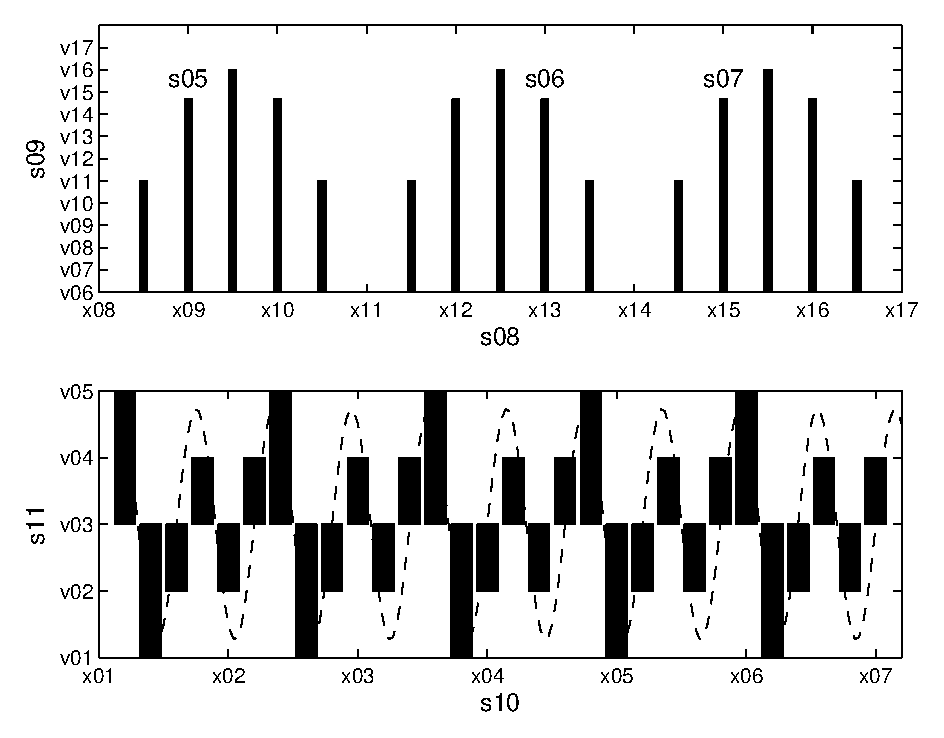
\includegraphics[width=0.9\textwidth]{figs/f_Qs_30_p_10_1.eps}}%
\end{psfrags}%
%
% End f_Qs_30_p_10_1.tex
\end{document}
% See http://www.mathworks.de/matlabcentral/fileexchange/loadFile.do?objectId=4638
% for recent versions of laprint.m.
%
% created by:           LaPrint version 3.16 (13.9.2004)
% created on:           12-Nov-2008 21:44:16
% eps bounding box:     17.5 cm x 13.125 cm
% comment:              
%
\begin{psfrags}%
\psfragscanon%
%
% text strings:
\psfrag{s05}[b][b]{{\tiny $\xi_{10}$}}%
\psfrag{s06}[b][b]{{\tiny $\xi_{50}$}}%
\psfrag{s07}[b][b]{{\tiny $\xi_{70}$}}%
\psfrag{s08}[t][t]{{\tiny $\nu$}}%
\psfrag{s09}[b][b]{{\tiny $\xi_{\nu}$}}%
\psfrag{s10}[t][t]{{\tiny Slot number}}%
\psfrag{s11}[b][b]{{\tiny $F_{slot}/\SI{}{A}$}}%
%
% xticklabels:
\psfrag{x01}[t][t]{{\tiny 0}}%
\psfrag{x02}[t][t]{{\tiny 5}}%
\psfrag{x03}[t][t]{{\tiny 10}}%
\psfrag{x04}[t][t]{{\tiny 15}}%
\psfrag{x05}[t][t]{{\tiny 20}}%
\psfrag{x06}[t][t]{{\tiny 25}}%
\psfrag{x07}[t][t]{{\tiny 30}}%
\psfrag{x08}[t][t]{{\tiny 0}}%
\psfrag{x09}[t][t]{{\tiny 10}}%
\psfrag{x10}[t][t]{{\tiny 20}}%
\psfrag{x11}[t][t]{{\tiny 30}}%
\psfrag{x12}[t][t]{{\tiny 40}}%
\psfrag{x13}[t][t]{{\tiny 50}}%
\psfrag{x14}[t][t]{{\tiny 60}}%
\psfrag{x15}[t][t]{{\tiny 70}}%
\psfrag{x16}[t][t]{{\tiny 80}}%
\psfrag{x17}[t][t]{{\tiny 90}}%
%
% yticklabels:
\psfrag{v01}[r][r]{{\tiny -1}}%
\psfrag{v02}[r][r]{{\tiny -0.5}}%
\psfrag{v03}[r][r]{{\tiny 0}}%
\psfrag{v04}[r][r]{{\tiny 0.5}}%
\psfrag{v05}[r][r]{{\tiny 1}}%
\psfrag{v06}[r][r]{{\tiny 0}}%
\psfrag{v07}[r][r]{{\tiny 0.1}}%
\psfrag{v08}[r][r]{{\tiny 0.2}}%
\psfrag{v09}[r][r]{{\tiny 0.3}}%
\psfrag{v10}[r][r]{{\tiny 0.4}}%
\psfrag{v11}[r][r]{{\tiny 0.5}}%
\psfrag{v12}[r][r]{{\tiny 0.6}}%
\psfrag{v13}[r][r]{{\tiny 0.7}}%
\psfrag{v14}[r][r]{{\tiny 0.8}}%
\psfrag{v15}[r][r]{{\tiny 0.9}}%
\psfrag{v16}[r][r]{{\tiny 1}}%
\psfrag{v17}[r][r]{{\tiny 1.1}}%
%
% Figure:

\subfloat[Slot mmf and winding factors\label{fig:f_Qs30_p10_1}]{%
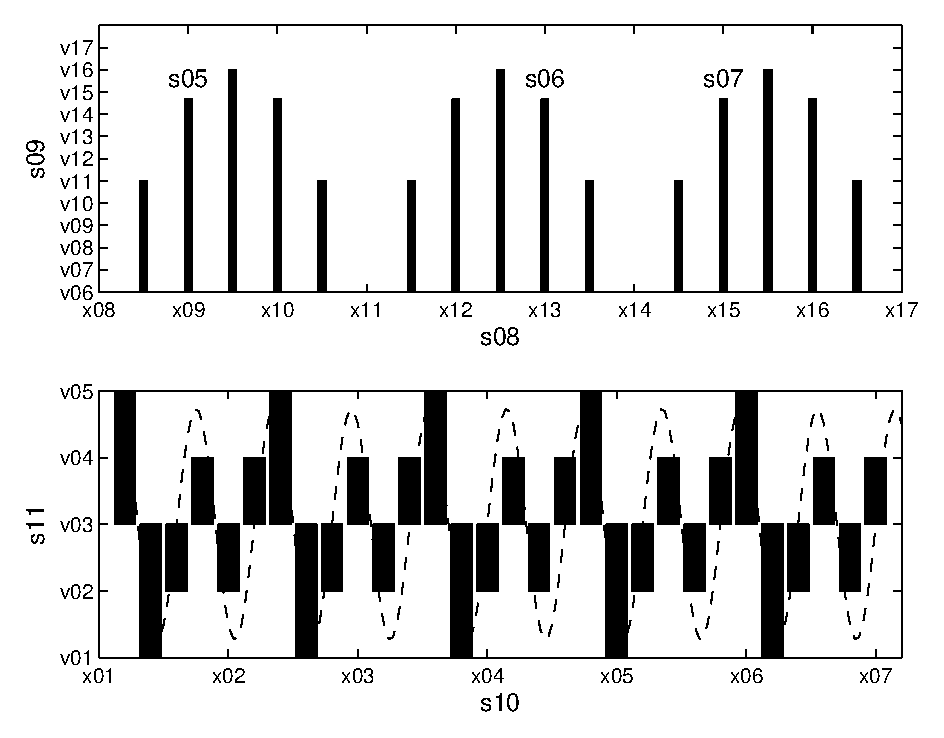
\includegraphics[width=0.9\textwidth]{figs/f_Qs_30_p_10_1.eps}}%
\end{psfrags}%
%
% End f_Qs_30_p_10_1.tex
}
  \caption{Non-overlapping single layer winding}
  \label{fig:Main_non-overlapping_single}
\end{figure}

\subsubsection{Double layer non-overlapping}
Fig.~\ref{fig:Main_non-overlapping_double}\subref{fig:dlw_yd_eq_1} shows a non-overlapping double layer winding. Each stator slot has two coil sides. Moreover, each slot needs to be assigned to a phase belt. 

The prototype stator with 30 slots is used with 10 pole pairs. This is a double layer winding and the number of slots is equal to the number of coils. Both $q$ and $q_c$ and the basic winding has 3 slots. The lowest harmonic has 10 pole pairs which is the same as the working harmonic. Therefore, the winding has no sub-harmonics. The matrix elements of the basic winding are 
\begin{equation}
  \mathbf{M_{1,b}} = 
  \begin{pmatrix}
  1&0&0\\
  0&0&1\\
  0&1&0\\ 
  \end{pmatrix} \
  \mathbf{M_{2,b}} = 
  \begin{pmatrix}
  0 &-1&0\\
  -1&0&0\\
  0&0&-1\\ 
  \end{pmatrix} 
\end{equation}
The winding factors and slot mmf are directly obtained from the winding matrix as shown in Fig.~\ref{fig:Main_non-overlapping_double}\subref{fig:f_Qs30_p10_2}. The current sheet that corresponds to the working harmonic is included.
\begin{figure}[htbp]
  \centering
  \fontsize{6}{6}\selectfont
  \subfloat[Winding layout\label{fig:dlw_yd_eq_1}]{%
  \begin{psfrags}%
\psfragscanon

% text strings:
\psfrag{t01}[bc]{{\tiny $y_d$}}
\psfrag{t02}[bl]{{\tiny Direction of coil assignment}}
\psfrag{t03}{{\tiny 1}}
\psfrag{t04}{{\tiny 2}}
\psfrag{t05}{{\tiny 3}}
\psfrag{t06}{{\tiny 4}}
\psfrag{t07}{{\tiny 5}}

% Figure:

\subfloat[Winding layout\label{fig:dlw_yd_eq_1}]{%
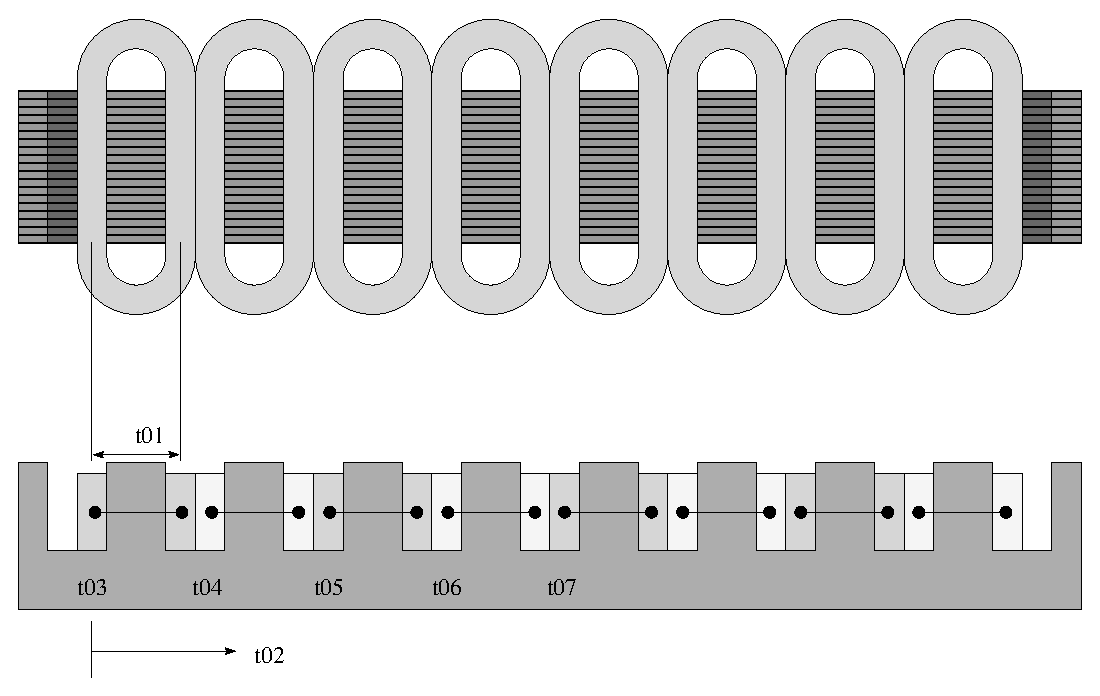
\includegraphics[height=7cm]{figs/f_double_layer_type2.eps}}
\end{psfrags}%
}
  \hfill
  \subfloat[Slot mmf and winding factors\label{fig:f_Qs30_p10_2}]{%  
  % This file is generated by the MATLAB m-file laprint.m. It can be included
% into LaTeX documents using the packages graphicx, color and psfrag.
% It is accompanied by a postscript file. A sample LaTeX file is:
%    \documentclass{article}\usepackage{graphicx,color,psfrag}
%    \begin{document}% This file is generated by the MATLAB m-file laprint.m. It can be included
% into LaTeX documents using the packages graphicx, color and psfrag.
% It is accompanied by a postscript file. A sample LaTeX file is:
%    \documentclass{article}\usepackage{graphicx,color,psfrag}
%    \begin{document}% This file is generated by the MATLAB m-file laprint.m. It can be included
% into LaTeX documents using the packages graphicx, color and psfrag.
% It is accompanied by a postscript file. A sample LaTeX file is:
%    \documentclass{article}\usepackage{graphicx,color,psfrag}
%    \begin{document}\input{f_Qs_30_p_10_2}\end{document}
% See http://www.mathworks.de/matlabcentral/fileexchange/loadFile.do?objectId=4638
% for recent versions of laprint.m.
%
% created by:           LaPrint version 3.16 (13.9.2004)
% created on:           12-Nov-2008 21:54:09
% eps bounding box:     17.5 cm x 13.125 cm
% comment:              
%
\begin{psfrags}%
\psfragscanon%
%
% text strings:
\psfrag{s05}[b][b]{$\xi_{10}$}
\psfrag{s06}[b][b]{$\xi_{50}$}
\psfrag{s07}[b][b]{$\xi_{70}$}
\psfrag{s08}[t][t]{$\nu$}
\psfrag{s09}[b][b]{$\xi_{\nu}$}
\psfrag{s10}[t][t]{Slot number}
\psfrag{s11}[b][b]{$F_{slot}/\SI{}{A}$}
%
% xticklabels:
\psfrag{x01}[t][t]{0}
\psfrag{x02}[t][t]{5}
\psfrag{x03}[t][t]{10}
\psfrag{x04}[t][t]{15}
\psfrag{x05}[t][t]{20}
\psfrag{x06}[t][t]{25}
\psfrag{x07}[t][t]{30}
\psfrag{x08}[t][t]{0}
\psfrag{x09}[t][t]{10}
\psfrag{x10}[t][t]{20}
\psfrag{x11}[t][t]{30}
\psfrag{x12}[t][t]{40}
\psfrag{x13}[t][t]{50}
\psfrag{x14}[t][t]{60}
\psfrag{x15}[t][t]{70}
\psfrag{x16}[t][t]{80}
\psfrag{x17}[t][t]{90}
%
% yticklabels:
\psfrag{v01}[r][r]{-2}
\psfrag{v02}[r][r]{-1}
\psfrag{v03}[r][r]{0}
\psfrag{v04}[r][r]{1}
\psfrag{v05}[r][r]{2}
\psfrag{v06}[r][r]{0}
\psfrag{v07}[r][r]{0.1}
\psfrag{v08}[r][r]{0.2}
\psfrag{v09}[r][r]{0.3}
\psfrag{v10}[r][r]{0.4}
\psfrag{v11}[r][r]{0.5}
\psfrag{v12}[r][r]{0.6}
\psfrag{v13}[r][r]{0.7}
\psfrag{v14}[r][r]{0.8}
\psfrag{v15}[r][r]{0.9}
\psfrag{v16}[r][r]{1}
\psfrag{v17}[r][r]{1.1}
%
% Figure:
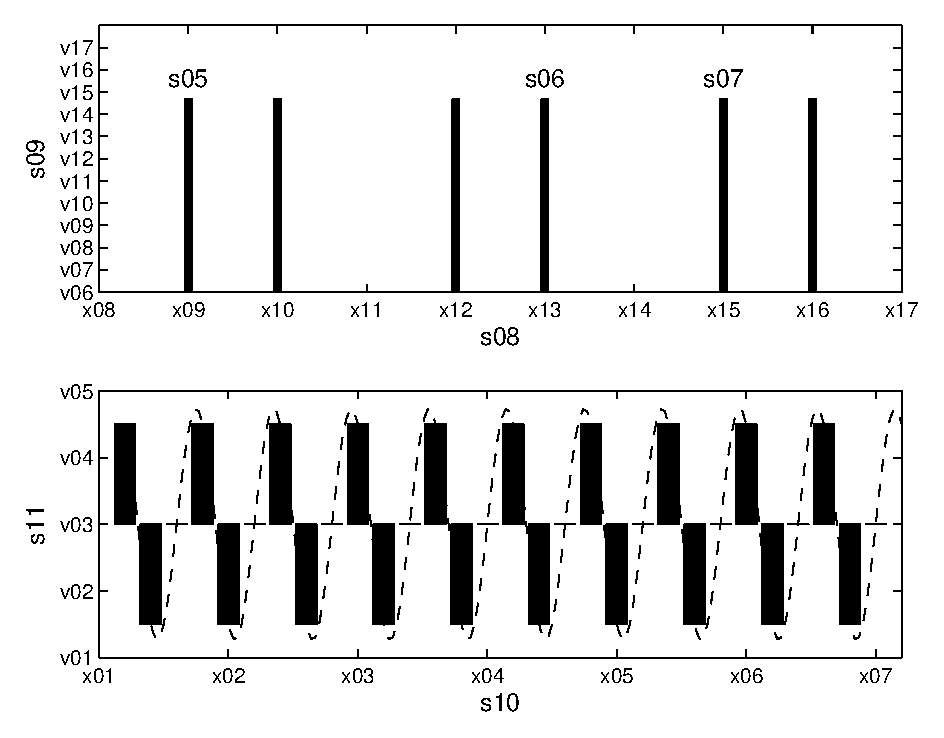
\includegraphics[width=0.47\textwidth]{figs/f_Qs_30_p_10_2.eps}
\end{psfrags}%
%
% End f_Qs_30_p_10_2.tex
\end{document}
% See http://www.mathworks.de/matlabcentral/fileexchange/loadFile.do?objectId=4638
% for recent versions of laprint.m.
%
% created by:           LaPrint version 3.16 (13.9.2004)
% created on:           12-Nov-2008 21:54:09
% eps bounding box:     17.5 cm x 13.125 cm
% comment:              
%
\begin{psfrags}%
\psfragscanon%
%
% text strings:
\psfrag{s05}[b][b]{$\xi_{10}$}
\psfrag{s06}[b][b]{$\xi_{50}$}
\psfrag{s07}[b][b]{$\xi_{70}$}
\psfrag{s08}[t][t]{$\nu$}
\psfrag{s09}[b][b]{$\xi_{\nu}$}
\psfrag{s10}[t][t]{Slot number}
\psfrag{s11}[b][b]{$F_{slot}/\SI{}{A}$}
%
% xticklabels:
\psfrag{x01}[t][t]{0}
\psfrag{x02}[t][t]{5}
\psfrag{x03}[t][t]{10}
\psfrag{x04}[t][t]{15}
\psfrag{x05}[t][t]{20}
\psfrag{x06}[t][t]{25}
\psfrag{x07}[t][t]{30}
\psfrag{x08}[t][t]{0}
\psfrag{x09}[t][t]{10}
\psfrag{x10}[t][t]{20}
\psfrag{x11}[t][t]{30}
\psfrag{x12}[t][t]{40}
\psfrag{x13}[t][t]{50}
\psfrag{x14}[t][t]{60}
\psfrag{x15}[t][t]{70}
\psfrag{x16}[t][t]{80}
\psfrag{x17}[t][t]{90}
%
% yticklabels:
\psfrag{v01}[r][r]{-2}
\psfrag{v02}[r][r]{-1}
\psfrag{v03}[r][r]{0}
\psfrag{v04}[r][r]{1}
\psfrag{v05}[r][r]{2}
\psfrag{v06}[r][r]{0}
\psfrag{v07}[r][r]{0.1}
\psfrag{v08}[r][r]{0.2}
\psfrag{v09}[r][r]{0.3}
\psfrag{v10}[r][r]{0.4}
\psfrag{v11}[r][r]{0.5}
\psfrag{v12}[r][r]{0.6}
\psfrag{v13}[r][r]{0.7}
\psfrag{v14}[r][r]{0.8}
\psfrag{v15}[r][r]{0.9}
\psfrag{v16}[r][r]{1}
\psfrag{v17}[r][r]{1.1}
%
% Figure:
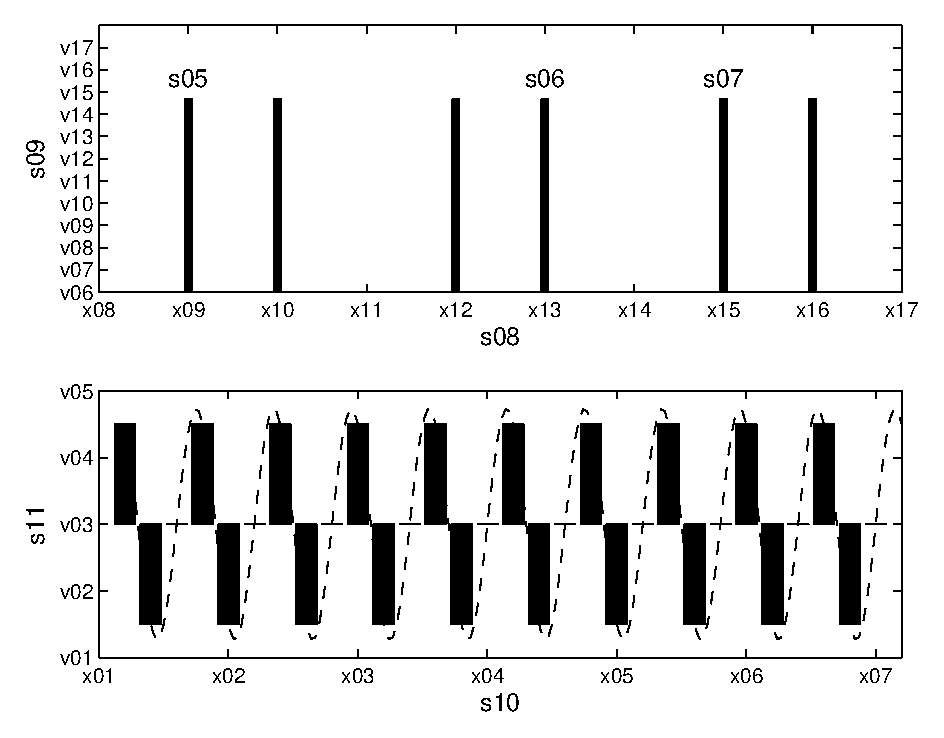
\includegraphics[width=0.47\textwidth]{figs/f_Qs_30_p_10_2.eps}
\end{psfrags}%
%
% End f_Qs_30_p_10_2.tex
\end{document}
% See http://www.mathworks.de/matlabcentral/fileexchange/loadFile.do?objectId=4638
% for recent versions of laprint.m.
%
% created by:           LaPrint version 3.16 (13.9.2004)
% created on:           12-Nov-2008 21:54:09
% eps bounding box:     17.5 cm x 13.125 cm
% comment:              
%
\begin{psfrags}%
\psfragscanon%
%
% text strings:
\psfrag{s05}[b][b]{$\xi_{10}$}
\psfrag{s06}[b][b]{$\xi_{50}$}
\psfrag{s07}[b][b]{$\xi_{70}$}
\psfrag{s08}[t][t]{$\nu$}
\psfrag{s09}[b][b]{$\xi_{\nu}$}
\psfrag{s10}[t][t]{Slot number}
\psfrag{s11}[b][b]{$F_{slot}/\SI{}{A}$}
%
% xticklabels:
\psfrag{x01}[t][t]{0}
\psfrag{x02}[t][t]{5}
\psfrag{x03}[t][t]{10}
\psfrag{x04}[t][t]{15}
\psfrag{x05}[t][t]{20}
\psfrag{x06}[t][t]{25}
\psfrag{x07}[t][t]{30}
\psfrag{x08}[t][t]{0}
\psfrag{x09}[t][t]{10}
\psfrag{x10}[t][t]{20}
\psfrag{x11}[t][t]{30}
\psfrag{x12}[t][t]{40}
\psfrag{x13}[t][t]{50}
\psfrag{x14}[t][t]{60}
\psfrag{x15}[t][t]{70}
\psfrag{x16}[t][t]{80}
\psfrag{x17}[t][t]{90}
%
% yticklabels:
\psfrag{v01}[r][r]{-2}
\psfrag{v02}[r][r]{-1}
\psfrag{v03}[r][r]{0}
\psfrag{v04}[r][r]{1}
\psfrag{v05}[r][r]{2}
\psfrag{v06}[r][r]{0}
\psfrag{v07}[r][r]{0.1}
\psfrag{v08}[r][r]{0.2}
\psfrag{v09}[r][r]{0.3}
\psfrag{v10}[r][r]{0.4}
\psfrag{v11}[r][r]{0.5}
\psfrag{v12}[r][r]{0.6}
\psfrag{v13}[r][r]{0.7}
\psfrag{v14}[r][r]{0.8}
\psfrag{v15}[r][r]{0.9}
\psfrag{v16}[r][r]{1}
\psfrag{v17}[r][r]{1.1}
%
% Figure:
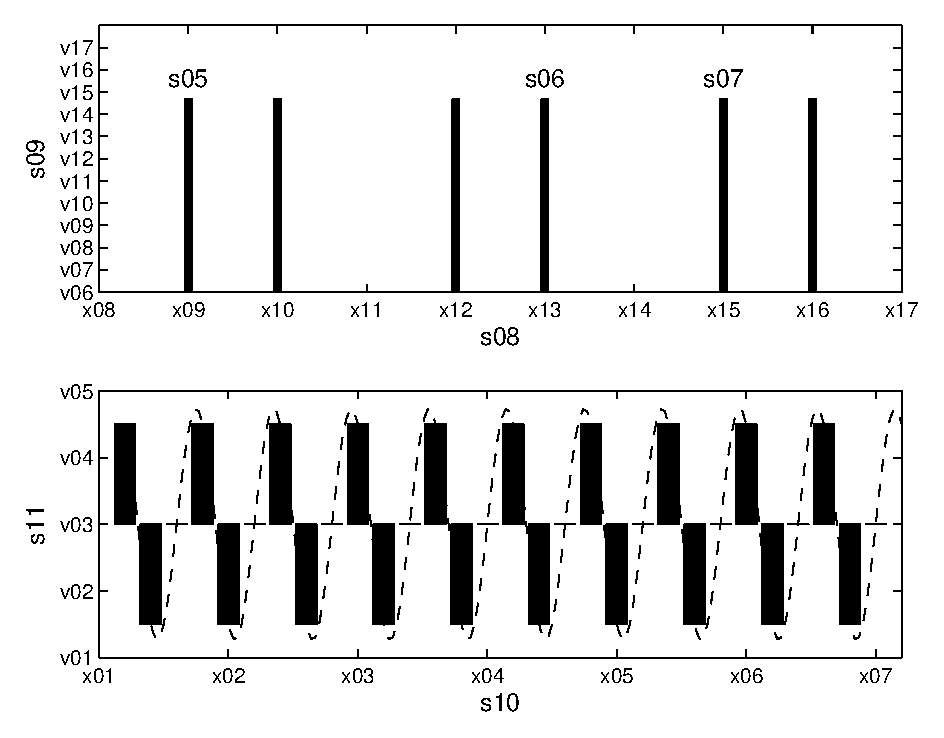
\includegraphics[width=0.47\textwidth]{figs/f_Qs_30_p_10_2.eps}
\end{psfrags}%
%
% End f_Qs_30_p_10_2.tex
}
  \caption{Non-overlapping double layer winding}
  \label{fig:Main_non-overlapping_double}
\end{figure}

\subsubsection{Single layer overlapping}
A general single layer overlapping winding is shown in~% 
Fig.~\ref{fig:Main_single_overlapping}\subref{fig:slw_yd_eq_1}. In this example the coil pitch equals 5. The ingoing coil side of the first coil is in slot 1 and the outgoing coil side in slot 6. It is clear from the figure that the coils overlap. 

The example to illustrate the slot mmf and current sheet has 30 slots and a pole pair number equal to 5. In Tab.~\ref{tab:Example_table} the average pole pitch equals the pole pitch. Therefore this is called a concentrated winding as determined from Fig.~\ref{fig:classification}. The basic winding matrix elements are given as
\begin{equation}
  \mathbf{M_{1,b}} = 
  \begin{pmatrix}
  1&0&0&-1&0&0\\    
  0&-1&0&0&1&0\\   
  0&0&1&0&0&-1\\   
  \end{pmatrix} \
  \mathbf{M_{2,b}} = 
  \begin{pmatrix}
  1& 0&0&-1&0&0\\
  0&-1&0& 0&1&0\\
  0& 0&1& 0&0&-1\\  
  \end{pmatrix} 
\end{equation}
The calculated winding factor along with the slot mmf and current sheet are shown in Fig.~\ref{fig:Main_single_overlapping}\subref{fig:f_Qs30_5_1}. It is important to mention that the coil sides are distributed in such a way as to obtain a sinusoidal slot mmf distribution. The number of slots per pole and phase can be increased to obtain a better sinusoidal distribution. In doing so, the harmonic content will become less.
\begin{figure}[htbp]
  \centering
  \fontsize{6}{6}\selectfont
  \subfloat[Single layer overlapping winding layout\label{fig:slw_yd_eq_1}]{%
  \begin{psfrags}%
\psfragscanon

% text strings:
\psfrag{t01}{{\tiny Coil pitch, $y_d$}}
\psfrag{t02}{{\tiny Overhang, $l_o$}}
\psfrag{t05}{{\tiny 1}}
\psfrag{t06}{{\tiny 2}}
\psfrag{t07}{{\tiny 3}}
\psfrag{t08}{{\tiny 4}}
\psfrag{t09}{{\tiny 5}}
\psfrag{t10}{{\tiny 6}}
\psfrag{t11}{{\tiny Direction of coil assignment}}

% Figure:

\subfloat[Single layer overlapping winding layout\label{fig:slw_yd_eq_1}]
  \hfill
  \subfloat[Slot mmf and winding factors\label{fig:f_Qs30_5_1}]{%
  % This file is generated by the MATLAB m-file laprint.m. It can be included
% into LaTeX documents using the packages graphicx, color and psfrag.
% It is accompanied by a postscript file. A sample LaTeX file is:
%    \documentclass{article}\usepackage{graphicx,color,psfrag}
%    \begin{document}% This file is generated by the MATLAB m-file laprint.m. It can be included
% into LaTeX documents using the packages graphicx, color and psfrag.
% It is accompanied by a postscript file. A sample LaTeX file is:
%    \documentclass{article}\usepackage{graphicx,color,psfrag}
%    \begin{document}% This file is generated by the MATLAB m-file laprint.m. It can be included
% into LaTeX documents using the packages graphicx, color and psfrag.
% It is accompanied by a postscript file. A sample LaTeX file is:
%    \documentclass{article}\usepackage{graphicx,color,psfrag}
%    \begin{document}\input{f_Qs_30_p_5_1}\end{document}
% See http://www.mathworks.de/matlabcentral/fileexchange/loadFile.do?objectId=4638
% for recent versions of laprint.m.
%
% created by:           LaPrint version 3.16 (13.9.2004)
% created on:           12-Nov-2008 21:46:31
% eps bounding box:     17.5 cm x 13.125 cm
% comment:              
%
\begin{psfrags}%
\psfragscanon%
%
% text strings:
\psfrag{s05}[b][b]{$\xi_{5}$}%
\psfrag{s06}[b][b]{$\xi_{25}$}%
\psfrag{s07}[b][b]{$\xi_{35}$}%
\psfrag{s08}[t][t]{$\nu$}%
\psfrag{s09}[b][b]{$\xi_{\nu}$}%
\psfrag{s10}[t][t]{Slot number}%
\psfrag{s11}[b][b]{$F_{slot}/\SI{}{A}$}%
%
% xticklabels:
\psfrag{x01}[t][t]{0}%
\psfrag{x02}[t][t]{5}%
\psfrag{x03}[t][t]{10}%
\psfrag{x04}[t][t]{15}%
\psfrag{x05}[t][t]{20}%
\psfrag{x06}[t][t]{25}%
\psfrag{x07}[t][t]{30}%
\psfrag{x08}[t][t]{0}%
\psfrag{x09}[t][t]{10}%
\psfrag{x10}[t][t]{20}%
\psfrag{x11}[t][t]{30}%
\psfrag{x12}[t][t]{40}%
\psfrag{x13}[t][t]{50}%
\psfrag{x14}[t][t]{60}%
%
% yticklabels:
\psfrag{v01}[r][r]{-1}%
\psfrag{v02}[r][r]{-0.5}%
\psfrag{v03}[r][r]{0}%
\psfrag{v04}[r][r]{0.5}%
\psfrag{v05}[r][r]{1}%
\psfrag{v06}[r][r]{0}%
\psfrag{v07}[r][r]{0.1}%
\psfrag{v08}[r][r]{0.2}%
\psfrag{v09}[r][r]{0.3}%
\psfrag{v10}[r][r]{0.4}%
\psfrag{v11}[r][r]{0.5}%
\psfrag{v12}[r][r]{0.6}%
\psfrag{v13}[r][r]{0.7}%
\psfrag{v14}[r][r]{0.8}%
\psfrag{v15}[r][r]{0.9}%
\psfrag{v16}[r][r]{1}%
\psfrag{v17}[r][r]{1.1}%
%
% Figure:

\subfloat[Slot mmf and winding factors\label{fig:f_Qs30_5_1}]{%
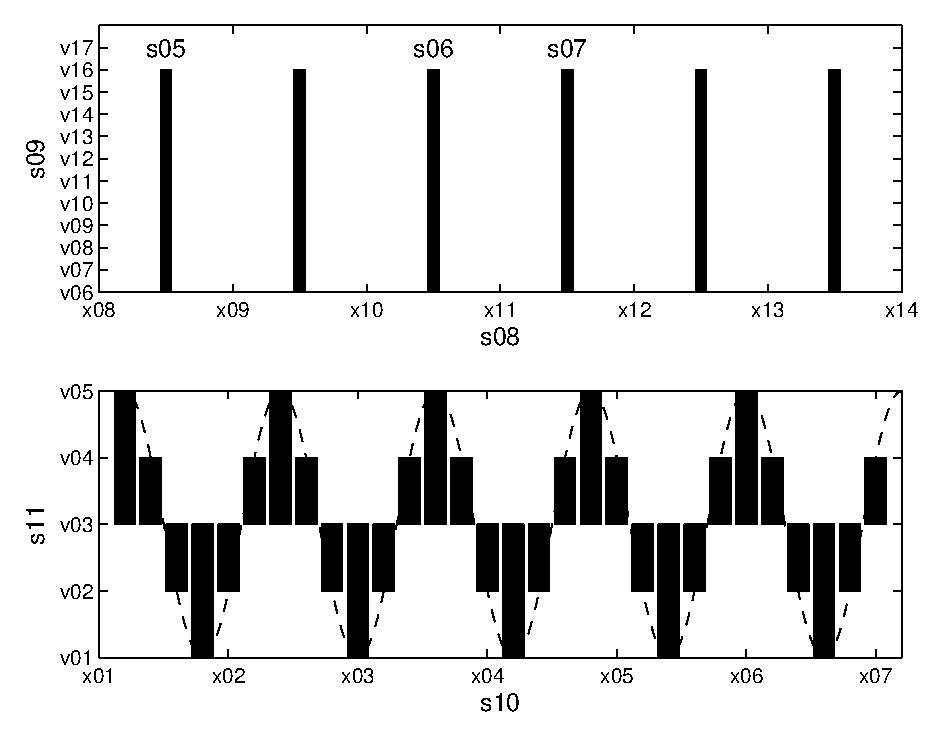
\includegraphics[width=0.9\textwidth]{figs/f_Qs_30_p_5_1.eps}}%
\end{psfrags}%
%
% End f_Qs_30_p_5_1.tex
\end{document}
% See http://www.mathworks.de/matlabcentral/fileexchange/loadFile.do?objectId=4638
% for recent versions of laprint.m.
%
% created by:           LaPrint version 3.16 (13.9.2004)
% created on:           12-Nov-2008 21:46:31
% eps bounding box:     17.5 cm x 13.125 cm
% comment:              
%
\begin{psfrags}%
\psfragscanon%
%
% text strings:
\psfrag{s05}[b][b]{$\xi_{5}$}%
\psfrag{s06}[b][b]{$\xi_{25}$}%
\psfrag{s07}[b][b]{$\xi_{35}$}%
\psfrag{s08}[t][t]{$\nu$}%
\psfrag{s09}[b][b]{$\xi_{\nu}$}%
\psfrag{s10}[t][t]{Slot number}%
\psfrag{s11}[b][b]{$F_{slot}/\SI{}{A}$}%
%
% xticklabels:
\psfrag{x01}[t][t]{0}%
\psfrag{x02}[t][t]{5}%
\psfrag{x03}[t][t]{10}%
\psfrag{x04}[t][t]{15}%
\psfrag{x05}[t][t]{20}%
\psfrag{x06}[t][t]{25}%
\psfrag{x07}[t][t]{30}%
\psfrag{x08}[t][t]{0}%
\psfrag{x09}[t][t]{10}%
\psfrag{x10}[t][t]{20}%
\psfrag{x11}[t][t]{30}%
\psfrag{x12}[t][t]{40}%
\psfrag{x13}[t][t]{50}%
\psfrag{x14}[t][t]{60}%
%
% yticklabels:
\psfrag{v01}[r][r]{-1}%
\psfrag{v02}[r][r]{-0.5}%
\psfrag{v03}[r][r]{0}%
\psfrag{v04}[r][r]{0.5}%
\psfrag{v05}[r][r]{1}%
\psfrag{v06}[r][r]{0}%
\psfrag{v07}[r][r]{0.1}%
\psfrag{v08}[r][r]{0.2}%
\psfrag{v09}[r][r]{0.3}%
\psfrag{v10}[r][r]{0.4}%
\psfrag{v11}[r][r]{0.5}%
\psfrag{v12}[r][r]{0.6}%
\psfrag{v13}[r][r]{0.7}%
\psfrag{v14}[r][r]{0.8}%
\psfrag{v15}[r][r]{0.9}%
\psfrag{v16}[r][r]{1}%
\psfrag{v17}[r][r]{1.1}%
%
% Figure:

\subfloat[Slot mmf and winding factors\label{fig:f_Qs30_5_1}]{%
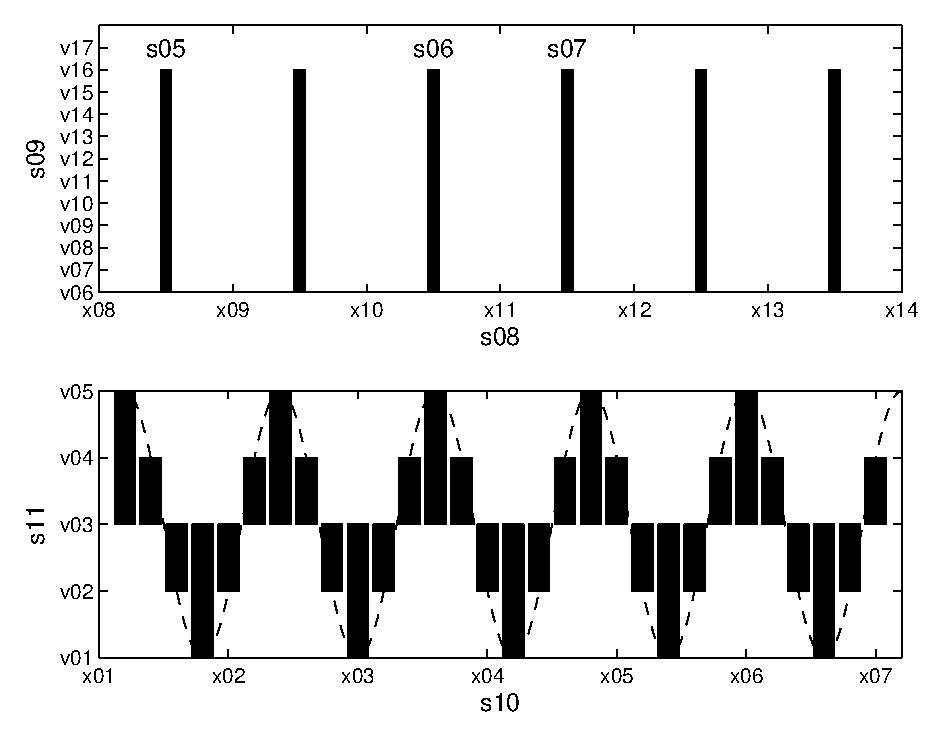
\includegraphics[width=0.9\textwidth]{figs/f_Qs_30_p_5_1.eps}}%
\end{psfrags}%
%
% End f_Qs_30_p_5_1.tex
\end{document}
% See http://www.mathworks.de/matlabcentral/fileexchange/loadFile.do?objectId=4638
% for recent versions of laprint.m.
%
% created by:           LaPrint version 3.16 (13.9.2004)
% created on:           12-Nov-2008 21:46:31
% eps bounding box:     17.5 cm x 13.125 cm
% comment:              
%
\begin{psfrags}%
\psfragscanon%
%
% text strings:
\psfrag{s05}[b][b]{$\xi_{5}$}%
\psfrag{s06}[b][b]{$\xi_{25}$}%
\psfrag{s07}[b][b]{$\xi_{35}$}%
\psfrag{s08}[t][t]{$\nu$}%
\psfrag{s09}[b][b]{$\xi_{\nu}$}%
\psfrag{s10}[t][t]{Slot number}%
\psfrag{s11}[b][b]{$F_{slot}/\SI{}{A}$}%
%
% xticklabels:
\psfrag{x01}[t][t]{0}%
\psfrag{x02}[t][t]{5}%
\psfrag{x03}[t][t]{10}%
\psfrag{x04}[t][t]{15}%
\psfrag{x05}[t][t]{20}%
\psfrag{x06}[t][t]{25}%
\psfrag{x07}[t][t]{30}%
\psfrag{x08}[t][t]{0}%
\psfrag{x09}[t][t]{10}%
\psfrag{x10}[t][t]{20}%
\psfrag{x11}[t][t]{30}%
\psfrag{x12}[t][t]{40}%
\psfrag{x13}[t][t]{50}%
\psfrag{x14}[t][t]{60}%
%
% yticklabels:
\psfrag{v01}[r][r]{-1}%
\psfrag{v02}[r][r]{-0.5}%
\psfrag{v03}[r][r]{0}%
\psfrag{v04}[r][r]{0.5}%
\psfrag{v05}[r][r]{1}%
\psfrag{v06}[r][r]{0}%
\psfrag{v07}[r][r]{0.1}%
\psfrag{v08}[r][r]{0.2}%
\psfrag{v09}[r][r]{0.3}%
\psfrag{v10}[r][r]{0.4}%
\psfrag{v11}[r][r]{0.5}%
\psfrag{v12}[r][r]{0.6}%
\psfrag{v13}[r][r]{0.7}%
\psfrag{v14}[r][r]{0.8}%
\psfrag{v15}[r][r]{0.9}%
\psfrag{v16}[r][r]{1}%
\psfrag{v17}[r][r]{1.1}%
%
% Figure:

\subfloat[Slot mmf and winding factors\label{fig:f_Qs30_5_1}]{%
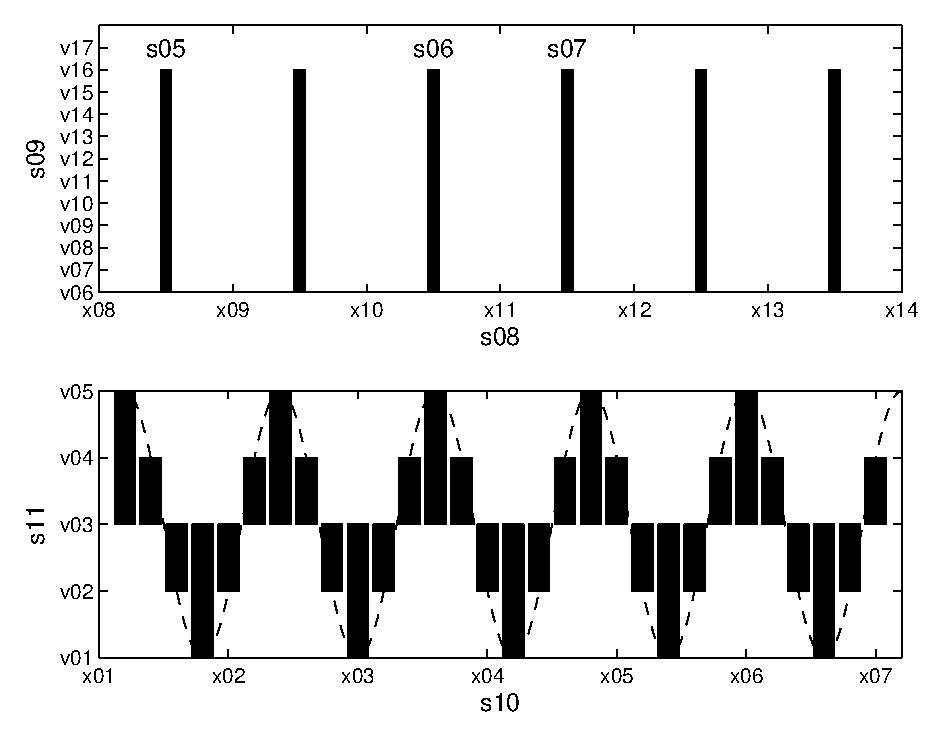
\includegraphics[width=0.9\textwidth]{figs/f_Qs_30_p_5_1.eps}}%
\end{psfrags}%
%
% End f_Qs_30_p_5_1.tex
}
  \caption{Single layer overlapping winding}
  \label{fig:Main_single_overlapping}
\end{figure}

\subsubsection{Double layer overlapping}
A double layer overlapping winding is commonly used in industrial machines. Overlapping double layer windings have a coil pitch greater than one, i.e.~$y_d>1$. Fig.~\ref{fig:dlw_yd_gt_1} shows a double layer winding. Starting at the first slot, the coils are inserted in a counter-clockwise direction. The first coil has its ingoing coil side in the bottom part of slot 1 and the return coil side is in the top part of slot 6. The phase belt constraint in \eqref{eqn:phase_belt_constraint} is used to determine the phase of the coil side in the bottom part of the slot while the top coil sides are given by the coil pitch $y_d$.

Fig.~\ref{fig:f_Qs30_p5_2} shows the slot mmf of a stator with $Q_s=30$ slots and $p=5$ pole pairs. Using the winding properties for this combination given in Tab.~\ref{tab:Example_table}, it is a concentrated winding. The winding has no sub-harmonics. 
\begin{figure}[htbp]
  \centering
  \fontsize{6}{6}\selectfont
  \subfloat[Double layer overlapping winding layout\label{fig:dlw_yd_gt_1}]{%
  \begin{psfrags}%
\psfragscanon

% text strings:
\psfrag{t01}{{\tiny Coil pitch, $y_d$}}
\psfrag{t02}{{\tiny Overhang, $l_o$}}
\psfrag{t03}{{\tiny Top}}
\psfrag{t04}{{\tiny Bottom}}
\psfrag{t05}{{\tiny 1}}
\psfrag{t06}{{\tiny 2}}
\psfrag{t07}{{\tiny 3}}
\psfrag{t08}{{\tiny 4}}
\psfrag{t09}{{\tiny 5}}
\psfrag{t10}{{\tiny 6}}
\psfrag{t11}{{\tiny Direction of coil assignment}}


% Figure:

\subfloat[Double layer overlapping winding layout\label{fig:dlw_yd_gt_1}]
  \hfill
  \subfloat[Slot mmf and winding factors\label{fig:f_Qs30_p5_2}]{%
  % This file is generated by the MATLAB m-file laprint.m. It can be included
% into LaTeX documents using the packages graphicx, color and psfrag.
% It is accompanied by a postscript file. A sample LaTeX file is:
%    \documentclass{article}\usepackage{graphicx,color,psfrag}
%    \begin{document}% This file is generated by the MATLAB m-file laprint.m. It can be included
% into LaTeX documents using the packages graphicx, color and psfrag.
% It is accompanied by a postscript file. A sample LaTeX file is:
%    \documentclass{article}\usepackage{graphicx,color,psfrag}
%    \begin{document}% This file is generated by the MATLAB m-file laprint.m. It can be included
% into LaTeX documents using the packages graphicx, color and psfrag.
% It is accompanied by a postscript file. A sample LaTeX file is:
%    \documentclass{article}\usepackage{graphicx,color,psfrag}
%    \begin{document}\input{f_Qs_30_p_5_2}\end{document}
% See http://www.mathworks.de/matlabcentral/fileexchange/loadFile.do?objectId=4638
% for recent versions of laprint.m.
%
% created by:           LaPrint version 3.16 (13.9.2004)
% created on:           12-Nov-2008 21:50:28
% eps bounding box:     17.5 cm x 13.125 cm
% comment:              
%
\begin{psfrags}%
\psfragscanon%
%
% text strings:
\psfrag{s05}[b][b]{{\tiny $\xi_{5}$}}%
\psfrag{s06}[b][b]{{\tiny $\xi_{25}$}}%
\psfrag{s07}[b][b]{{\tiny $\xi_{35}$}}%
\psfrag{s08}[t][t]{{\tiny $\nu$}}%
\psfrag{s09}[b][b]{{\tiny $\xi_{\nu}$}}%
\psfrag{s10}[t][t]{{\tiny Slot number}}%
\psfrag{s11}[b][b]{{\tiny $F_{slot}/\SI{}{A}$}}%
%
% xticklabels:
\psfrag{x01}[t][t]{{\tiny 0}}%
\psfrag{x02}[t][t]{{\tiny 5}}%
\psfrag{x03}[t][t]{{\tiny 10}}%
\psfrag{x04}[t][t]{{\tiny 15}}%
\psfrag{x05}[t][t]{{\tiny 20}}%
\psfrag{x06}[t][t]{{\tiny 25}}%
\psfrag{x07}[t][t]{{\tiny 30}}%
\psfrag{x08}[t][t]{{\tiny 0}}%
\psfrag{x09}[t][t]{{\tiny 10}}%
\psfrag{x10}[t][t]{{\tiny 20}}%
\psfrag{x11}[t][t]{{\tiny 30}}%
\psfrag{x12}[t][t]{{\tiny 40}}%
\psfrag{x13}[t][t]{{\tiny 50}}%
\psfrag{x14}[t][t]{{\tiny 60}}%
%
% yticklabels:
\psfrag{v01}[r][r]{{\tiny -2}}%
\psfrag{v02}[r][r]{{\tiny -1}}%
\psfrag{v03}[r][r]{{\tiny 0}}%
\psfrag{v04}[r][r]{{\tiny 1}}%
\psfrag{v05}[r][r]{{\tiny 2}}%
\psfrag{v06}[r][r]{{\tiny 0}}%
\psfrag{v07}[r][r]{{\tiny 0.1}}%
\psfrag{v08}[r][r]{{\tiny 0.2}}%
\psfrag{v09}[r][r]{{\tiny 0.3}}%
\psfrag{v10}[r][r]{{\tiny 0.4}}%
\psfrag{v11}[r][r]{{\tiny 0.5}}%
\psfrag{v12}[r][r]{{\tiny 0.6}}%
\psfrag{v13}[r][r]{{\tiny 0.7}}%
\psfrag{v14}[r][r]{{\tiny 0.8}}%
\psfrag{v15}[r][r]{{\tiny 0.9}}%
\psfrag{v16}[r][r]{{\tiny 1}}%
\psfrag{v17}[r][r]{{\tiny 1.1}}%
%
% Figure:

\subfloat[Slot mmf and winding factors\label{fig:f_Qs30_p5_2}]{%
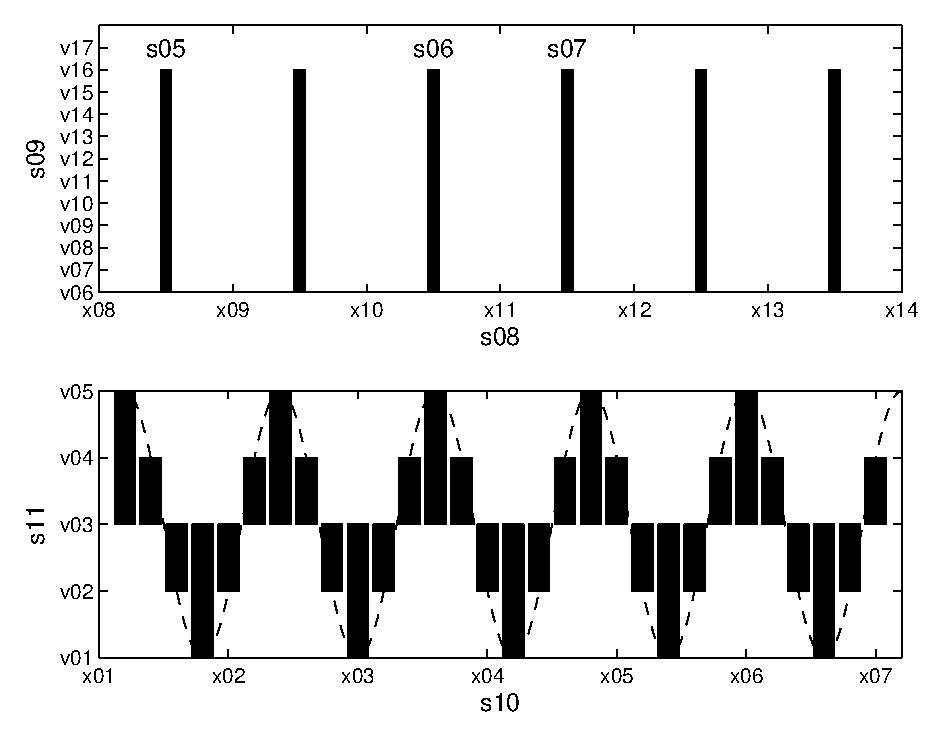
\includegraphics[width=0.9\textwidth]{figs/f_Qs_30_p_5_2.eps}}%
\end{psfrags}%
%
% End f_Qs_30_p_5_2.tex
\end{document}
% See http://www.mathworks.de/matlabcentral/fileexchange/loadFile.do?objectId=4638
% for recent versions of laprint.m.
%
% created by:           LaPrint version 3.16 (13.9.2004)
% created on:           12-Nov-2008 21:50:28
% eps bounding box:     17.5 cm x 13.125 cm
% comment:              
%
\begin{psfrags}%
\psfragscanon%
%
% text strings:
\psfrag{s05}[b][b]{{\tiny $\xi_{5}$}}%
\psfrag{s06}[b][b]{{\tiny $\xi_{25}$}}%
\psfrag{s07}[b][b]{{\tiny $\xi_{35}$}}%
\psfrag{s08}[t][t]{{\tiny $\nu$}}%
\psfrag{s09}[b][b]{{\tiny $\xi_{\nu}$}}%
\psfrag{s10}[t][t]{{\tiny Slot number}}%
\psfrag{s11}[b][b]{{\tiny $F_{slot}/\SI{}{A}$}}%
%
% xticklabels:
\psfrag{x01}[t][t]{{\tiny 0}}%
\psfrag{x02}[t][t]{{\tiny 5}}%
\psfrag{x03}[t][t]{{\tiny 10}}%
\psfrag{x04}[t][t]{{\tiny 15}}%
\psfrag{x05}[t][t]{{\tiny 20}}%
\psfrag{x06}[t][t]{{\tiny 25}}%
\psfrag{x07}[t][t]{{\tiny 30}}%
\psfrag{x08}[t][t]{{\tiny 0}}%
\psfrag{x09}[t][t]{{\tiny 10}}%
\psfrag{x10}[t][t]{{\tiny 20}}%
\psfrag{x11}[t][t]{{\tiny 30}}%
\psfrag{x12}[t][t]{{\tiny 40}}%
\psfrag{x13}[t][t]{{\tiny 50}}%
\psfrag{x14}[t][t]{{\tiny 60}}%
%
% yticklabels:
\psfrag{v01}[r][r]{{\tiny -2}}%
\psfrag{v02}[r][r]{{\tiny -1}}%
\psfrag{v03}[r][r]{{\tiny 0}}%
\psfrag{v04}[r][r]{{\tiny 1}}%
\psfrag{v05}[r][r]{{\tiny 2}}%
\psfrag{v06}[r][r]{{\tiny 0}}%
\psfrag{v07}[r][r]{{\tiny 0.1}}%
\psfrag{v08}[r][r]{{\tiny 0.2}}%
\psfrag{v09}[r][r]{{\tiny 0.3}}%
\psfrag{v10}[r][r]{{\tiny 0.4}}%
\psfrag{v11}[r][r]{{\tiny 0.5}}%
\psfrag{v12}[r][r]{{\tiny 0.6}}%
\psfrag{v13}[r][r]{{\tiny 0.7}}%
\psfrag{v14}[r][r]{{\tiny 0.8}}%
\psfrag{v15}[r][r]{{\tiny 0.9}}%
\psfrag{v16}[r][r]{{\tiny 1}}%
\psfrag{v17}[r][r]{{\tiny 1.1}}%
%
% Figure:

\subfloat[Slot mmf and winding factors\label{fig:f_Qs30_p5_2}]{%
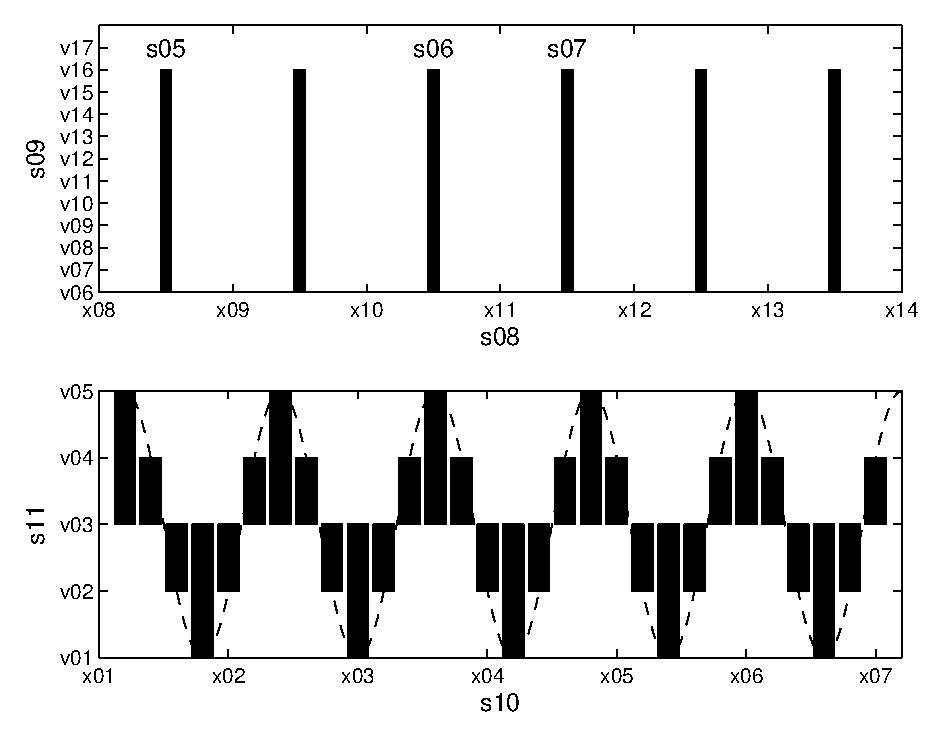
\includegraphics[width=0.9\textwidth]{figs/f_Qs_30_p_5_2.eps}}%
\end{psfrags}%
%
% End f_Qs_30_p_5_2.tex
\end{document}
% See http://www.mathworks.de/matlabcentral/fileexchange/loadFile.do?objectId=4638
% for recent versions of laprint.m.
%
% created by:           LaPrint version 3.16 (13.9.2004)
% created on:           12-Nov-2008 21:50:28
% eps bounding box:     17.5 cm x 13.125 cm
% comment:              
%
\begin{psfrags}%
\psfragscanon%
%
% text strings:
\psfrag{s05}[b][b]{{\tiny $\xi_{5}$}}%
\psfrag{s06}[b][b]{{\tiny $\xi_{25}$}}%
\psfrag{s07}[b][b]{{\tiny $\xi_{35}$}}%
\psfrag{s08}[t][t]{{\tiny $\nu$}}%
\psfrag{s09}[b][b]{{\tiny $\xi_{\nu}$}}%
\psfrag{s10}[t][t]{{\tiny Slot number}}%
\psfrag{s11}[b][b]{{\tiny $F_{slot}/\SI{}{A}$}}%
%
% xticklabels:
\psfrag{x01}[t][t]{{\tiny 0}}%
\psfrag{x02}[t][t]{{\tiny 5}}%
\psfrag{x03}[t][t]{{\tiny 10}}%
\psfrag{x04}[t][t]{{\tiny 15}}%
\psfrag{x05}[t][t]{{\tiny 20}}%
\psfrag{x06}[t][t]{{\tiny 25}}%
\psfrag{x07}[t][t]{{\tiny 30}}%
\psfrag{x08}[t][t]{{\tiny 0}}%
\psfrag{x09}[t][t]{{\tiny 10}}%
\psfrag{x10}[t][t]{{\tiny 20}}%
\psfrag{x11}[t][t]{{\tiny 30}}%
\psfrag{x12}[t][t]{{\tiny 40}}%
\psfrag{x13}[t][t]{{\tiny 50}}%
\psfrag{x14}[t][t]{{\tiny 60}}%
%
% yticklabels:
\psfrag{v01}[r][r]{{\tiny -2}}%
\psfrag{v02}[r][r]{{\tiny -1}}%
\psfrag{v03}[r][r]{{\tiny 0}}%
\psfrag{v04}[r][r]{{\tiny 1}}%
\psfrag{v05}[r][r]{{\tiny 2}}%
\psfrag{v06}[r][r]{{\tiny 0}}%
\psfrag{v07}[r][r]{{\tiny 0.1}}%
\psfrag{v08}[r][r]{{\tiny 0.2}}%
\psfrag{v09}[r][r]{{\tiny 0.3}}%
\psfrag{v10}[r][r]{{\tiny 0.4}}%
\psfrag{v11}[r][r]{{\tiny 0.5}}%
\psfrag{v12}[r][r]{{\tiny 0.6}}%
\psfrag{v13}[r][r]{{\tiny 0.7}}%
\psfrag{v14}[r][r]{{\tiny 0.8}}%
\psfrag{v15}[r][r]{{\tiny 0.9}}%
\psfrag{v16}[r][r]{{\tiny 1}}%
\psfrag{v17}[r][r]{{\tiny 1.1}}%
%
% Figure:

\subfloat[Slot mmf and winding factors\label{fig:f_Qs30_p5_2}]{%
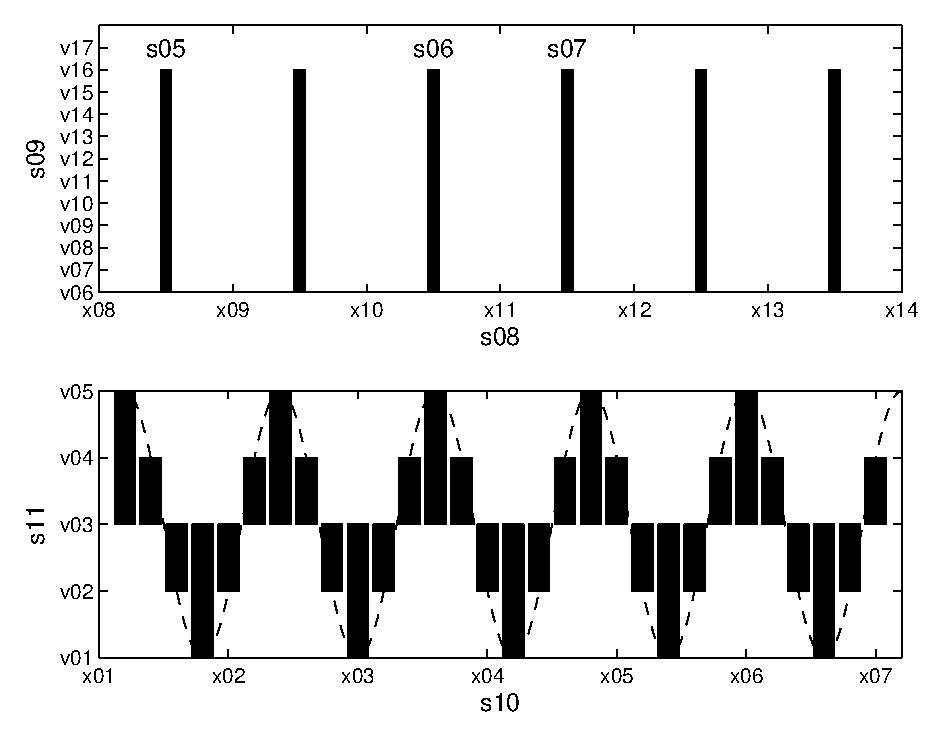
\includegraphics[width=0.9\textwidth]{figs/f_Qs_30_p_5_2.eps}}%
\end{psfrags}%
%
% End f_Qs_30_p_5_2.tex
}
  \caption{Double layer overlapping winding}
  \label{Main_double_overlapping}
\end{figure}

\clearpage
\section{Summary}
In this report an algorithm was derived to present a winding in a matrix form. This compact form allows the calculation of the winding factors for all harmonics. The basis of the algorithm is the phase belt sequence and the phase belt constraint which are derived from the air gap mmf envelope functions. 

\begin{figure}[htbp]
  \centering
  \fontsize{8}{6}\selectfont
  \begin{overpic}[scale=1.5,grid]
  {figs/f_double_layer_ex}
  \put(6.3,7.2){+1}  
  \put(6.3,10.8){+1}
  \put(16,7.2){-2}
  \put(16,10.8){-2}
  \put(25.6,7.2){+3}
  \put(25.6,10.8){+3}
  \put(35.2,7.2){-1}  
  \put(35.2,10.8){-1}
  \put(44.5,7.2){+2}
  \put(44.5,10.8){+2}
  \put(54.1,7.2){-3}
  \put(54.1,10.8){-3}
  \put(6.5,3){$\tau_s=\SI{12}{\arcdeg}$}
  \put(6.5,17){$\SI{0}{\arcdeg}$}  
  \dashline{1}(7,20)(7.5,78)
  \put(19.8,17){$\SI{18}{\arcdeg}$}  
  \dashline{1}(21,20)(21,78)
  \end{overpic}
  \caption{Double layer overlapping winding}
  \label{Main_double_overlapping}
\end{figure}